\section{Theoretical Proofs and Structural Properties}
\label{app:proofs}

This appendix collects proofs, structural properties, and auxiliary analysis for \starname{}.
Theorem~\ref{thm:recovery} is stated in the main text, while its full proof and related structural results are given here.
We also provide additional analysis of blackboard accumulation, routing length, the precision--coverage trade-off of $\alpha$, and connections to hierarchical control.

\subsection{Proof of Theorem~\ref{thm:recovery}}
\label{app:proof_recovery}

\begin{proof}[Proof of Theorem~\ref{thm:recovery}]
By Eq.~(\ref{eq:count_tensor}), the weighted count tensor under parameter $\alpha$ is
\[
\mathbf{C}^{\alpha}[a,s,t,a']
=
\sum_i \sum_j
\bigl(r_i+\alpha(1-r_i)\bigr)\,
\indicator\!\bigl[a^{(i)}_j=a,\; s^{(i)}_j=s,\; t_i=t,\; a^{(i)}_{j+1}=a'\bigr].
\]
For $\alpha>0$, both successful traces ($r_i=1$) and unsuccessful traces ($r_i=0$) contribute non-zero weight.
Hence, for any fixed error-state triple $(a,s,t)$ with $s\in\{\sfail,\sblock,\smiss\}$, the support of $\mathbf{C}^{\alpha}[a,s,t,\cdot]$ includes every successor observed in either successful or unsuccessful traces traversing that state.
After row normalization, the same support is inherited by $\mathbf{M}^{\alpha}[a,s,t,\cdot]$.

In contrast, when $\alpha=0$, unsuccessful traces contribute zero weight, so
\[
\mathbf{C}^{0}[a,s,t,a']
=
\sum_i \sum_j
r_i\,
\indicator\!\bigl[a^{(i)}_j=a,\; s^{(i)}_j=s,\; t_i=t,\; a^{(i)}_{j+1}=a'\bigr].
\]
Therefore, the support of $\mathbf{M}^{0}[a,s,t,\cdot]$ contains only successors observed in successful traces.

It follows immediately that
\[
\bigl|\,\textup{supp}\, \mathbf{M}^{\alpha}[a,s,t,\cdot]\bigr|
\ge
\bigl|\,\textup{supp}\, \mathbf{M}^{0}[a,s,t,\cdot]\bigr|.
\]
Moreover, if at least one unsuccessful trace traverses $(a,s,t)$ and contributes a successor not observed in successful traces, then the containment is strict, yielding
\[
\bigl|\,\textup{supp}\, \mathbf{M}^{\alpha}[a,s,t,\cdot]\bigr|
>
\bigl|\,\textup{supp}\, \mathbf{M}^{0}[a,s,t,\cdot]\bigr|.
\]
This proves the claim.
\end{proof}

\subsection{Blackboard Filtration and Information Non-Decrease}
\label{app:thm_info}

\begin{theorem}[Information Non-Decrease]
\label{thm:info}
Let $Y$ be the answer random variable and $\Board_k$ the blackboard state at step $k$.  The blackboard filtration satisfies $I(Y;\, \Board_k) \leq I(Y;\, \Board_{k+1})$ for all $0 \leq k < K$.
\end{theorem}

\begin{proof}
Let $Y$ denote the answer random variable and $\Board_k$ the blackboard at step $k$.  By construction the blackboard is append-only, so $\Board_k \subseteq \Board_{k+1}$.  Write $\Board_{k+1} = (\Board_k, \Delta_k)$ where $\Delta_k = \Board_{k+1} \setminus \Board_k$.

By the chain rule for mutual information:
\begin{equation}
    I(Y;\, \Board_{k+1}) = I(Y;\, \Board_k, \Delta_k) = I(Y;\, \Board_k) + I(Y;\, \Delta_k \mid \Board_k)
\end{equation}

Since mutual information is non-negative, $I(Y;\, \Delta_k \mid \Board_k) \geq 0$, and therefore:
\begin{equation}
    I(Y;\, \Board_{k+1}) \geq I(Y;\, \Board_k)
\end{equation}

Equality holds iff $\Delta_k \perp Y \mid \Board_k$---the new outputs are conditionally independent of the answer given existing evidence.  By induction, $I(Y;\, \Board_0) \leq \cdots \leq I(Y;\, \Board_K)$.
\end{proof}

\begin{corollary}[Fusion Sufficiency]
\label{cor:fusion}
The fusion agent operates on $\Board_K \supseteq \{(a, m^*_a(\theta_a))\}$ for all executed agents $a$.  Therefore:
\begin{equation}
    I(Y;\, \Board_K) \geq I(Y;\, \phi_a(\Board_0, q)) \quad \forall\, a \text{ executed}
\end{equation}
The multi-agent pipeline provides at least as much information about $Y$ as any single-agent baseline with access to only one agent's output.
\end{corollary}

\begin{remark}[Sufficiency vs.\ exploitation]
While $\Board_K$ is a sufficient statistic among all functions of the agent outputs, the LLM-based fusion function $F(\Board_K, q)$ may not exploit all information.  The gap $I(Y; \Board_K) - I(Y; F(\Board_K, q))$ is the residual that motivates future work on fusion-stage improvement.
\end{remark}

\subsection{Bounded Routing Length}
\label{app:thm_convergence}

\begin{theorem}[Bounded Convergence]
\label{thm:convergence}
The routing process in Algorithm~\ref{alg:execution} terminates in at most $\min(T, |\Agents^{(1)}| + 2)$ steps.
\end{theorem}

\begin{proof}
Termination in $K^* \leq \min(T, |\Agents^{(1)}| + 2)$ steps is shown as follows.

\textbf{Case 1 (Nominal).}  Under System~1, $\sigma_t$ defines an acyclic path from $a_{\shead}$ through a subset of $\Agents^{(1)}$ to $a_{\sfuse}$.  Path length $\leq |\Agents^{(1)}| + 2$.

\textbf{Case 2 (With retirements).}  Each agent producing \sfail enters $\mathcal{F}$ (Algorithm~\ref{alg:execution}, line~11) and is excluded from $\Agents_\text{next}$ (line~5).  Each retirement eliminates $\geq 1$ agent.  After at most $|\Agents^{(1)}|$ retirements, the safety net routes to $a_{\sfuse}$.

\textbf{Case 3 (Budget).}  The explicit cap $T$ ensures termination regardless.

Combined: $K^* \leq \min(T, |\Agents^{(1)}| + 2) = \min(T, 8)$ with the \starname{} agent pool.
\end{proof}

\begin{proposition}[Expected Step Count]
\label{prop:steps}
Let $p_s$ denote the average specialist success rate and $d$ the path length for task type $t$.  The expected routing steps are:
\begin{equation}
    \Expect[K] \approx d + 2 + (1-p_s) \cdot \bar{R}
\end{equation}
where $\bar{R}$ is the mean recovery path length.  With empirical rates $p_s \approx 0.82$ (STARK), $0.65$ (STB24), $0.55$ (STB26), $\Expect[K] \in [3.2, 4.8]$---well below the bound of~8.
\end{proposition}

\subsection{Precision--Coverage Trade-off of $\alpha$}
\label{app:alpha}

Theorem~\ref{thm:recovery} shows that $\alpha > 0$ is necessary for the matrix to have non-empty recovery support on error states.
This subsection characterizes the trade-off introduced by $\alpha$: as more unsuccessful traces are retained, recovery coverage improves while nominal-path precision may degrade.

\begin{proposition}[Precision--Coverage Trade-off of $\alpha$]
\label{prop:alpha}
Define routing precision and recovery coverage as
\begin{align}
\text{Prec}(\alpha) &= \Expect_{(a,s,t) \sim \Omega_1}\bigl[\pi_2(a^* \mid a, s, t)\bigr], \\
\text{Cov}(\alpha) &= \frac{1}{|\Omega_2|}\sum_{(a,s,t) \in \Omega_2} \indicator\bigl[\exists\, a': \mathbf{M}^\alpha[a,s,t,a'] > 0\bigr],
\end{align}
where $a^*$ denotes the optimal successor under an oracle policy and $\Omega_2$ the set of error-state triples.
Then $\text{Prec}(\alpha)$ is non-increasing in $\alpha$, $\text{Cov}(\alpha)$ is non-decreasing, and the parameter $\alpha$ smoothly interpolates between maximum routing precision ($\alpha \to 0$, zero recovery coverage) and maximum recovery coverage ($\alpha \to 1$, noisy nominal routing).
\end{proposition}

\begin{proof}[Proof sketch]
Increasing $\alpha$ strictly enlarges the support of every error-state row (Theorem~\ref{thm:recovery}), proving the coverage monotonicity.
For precision, consider a nominal state $(a, s, t) \in \Omega_1$ where the optimal successor $a^*$ is the most-observed successor in successful traces; as $\alpha$ grows, unsuccessful-trace transitions to non-optimal successors $a' \neq a^*$ receive relatively more mass in the row normalization, decreasing the normalized probability of $a^*$.
\end{proof}

\begin{figure}[H]
\centering
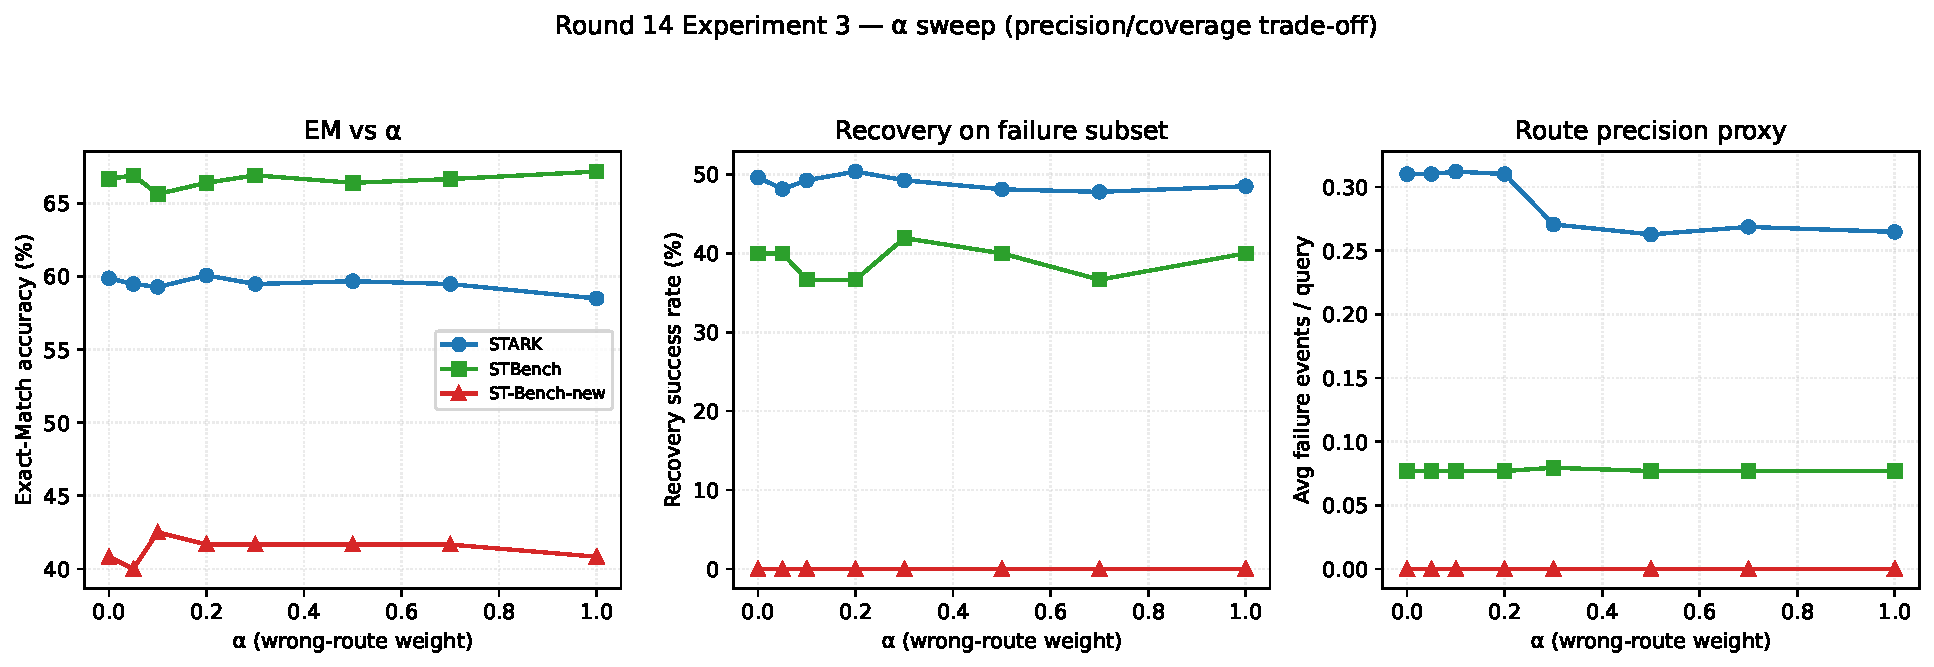
\includegraphics[width=0.85\textwidth]{figures/alpha_sweep.pdf}
\caption{Empirical precision--coverage trade-off of $\alpha$ across three benchmarks (Qwen3-8B, balanced slice).  Sweeping $\alpha \in [0, 1]$ confirms Proposition~\ref{prop:alpha}: recovery coverage is non-decreasing in $\alpha$ while overall accuracy degrades only gently over the useful range.  The operating point $\alpha = 0.3$ used throughout the main text sits in the plateau region where recovery transitions are populated without materially perturbing nominal-path routing.  The $\alpha = 0$ configuration (success-only training) corresponds to the empty-support regime of Theorem~\ref{thm:recovery}.}
\label{fig:alpha_sweep}
\end{figure}

\subsection{Parallel Execution Speedup}
\label{app:parallel}

\begin{proposition}[Scatter-Gather Speedup]
\label{prop:speedup}
At step $k$, let $m = |\Agents_k|$ agents execute with individual times $\{T_a\}$.  Sequential execution requires $T_\text{seq} = \sum_a T_a$.  Parallel scatter-gather requires:
\begin{equation}
    T_\text{par} = \max_a T_a + T_\text{oh}, \qquad S = \frac{T_\text{seq}}{T_\text{par}} \leq m
\end{equation}
where $T_\text{oh}$ is scheduling overhead.  Since deterministic computations execute in $<$10ms and LLM inference dominates at 1--5s, $T_\text{oh} \ll T_a$ and speedup approaches $m$ for homogeneous latencies.
\end{proposition}

\subsection{Extract--Compute--Deposit as Information Channel}
\label{app:channel}

Each agent $a$ can be modeled as a noisy channel from query $q$ to blackboard entry $b_a$:
\begin{equation}
    q \xrightarrow[\text{(noisy)}]{\texttt{extract}} \theta \xrightarrow[\text{(exact)}]{\texttt{compute}} m^*(\theta) = b_a
\end{equation}
The extraction step is the noisy component (the LLM may extract incorrect parameters); the computation step is noiseless (deterministic solver).  The channel capacity is:
\begin{equation}
    C_a = \max_{p(q)} I(q;\, b_a)
\end{equation}
Since $b_a = m^*(\theta)$ is deterministic, $H(b_a \mid \theta) = 0$, and so $I(q; b_a) = I(q; \theta)$ when $m^*$ is injective.  The bottleneck is \emph{entirely in extraction}: improving parameter extraction directly improves channel capacity, while computation accuracy is guaranteed by construction.  This formalizes why \starname{} achieves near-perfect accuracy on computation-intensive tasks---the extraction problem (``which parameters?'') is much simpler than the original computation problem.

\subsection{Connection to Hierarchical Reinforcement Learning}
\label{app:hrl}

\starname{}'s routing admits a natural interpretation through the lens of options.  Each agent $a$ corresponds to an option with:
\begin{itemize}
    \item \textbf{Initiation set}: $\mathcal{I}_a = \{(a',s,t): \pi(a \mid a',s,t) > 0\}$
    \item \textbf{Policy}: the extract--compute--deposit protocol $\phi_a$
    \item \textbf{Termination}: single-step (the agent always terminates after one execution)
\end{itemize}
The kernel $\pi$ is a \emph{policy over options}, and the dual-system decomposition combines a hand-crafted policy (System~1) with a learned one (System~2).

Unlike standard options, \starname{}'s agents are deterministic in their computation and stochastic only in parameter extraction (the LLM component).  This separation suggests the matrix could be further refined via reinforcement learning---optimizing transition probabilities directly against task accuracy---bridging trace-based training and reward-based optimization.

%% ============================================================
\FloatBarrier
\section{STB24 Comparison with Published Baselines}
\label{app:published}

Table~\ref{tab:published} compares \starname{} (Qwen3-8B, 8B parameters, local) against published GPT-4o results on STB24 from~\citep{li2025stbench}.
Open-7B$^\ddagger$ denotes the best reported open-source 7B-class model from the same source.

\begin{table}[!htbp]
\centering
\caption{STB24: \starname{} vs.\ published baselines. $\uparrow$/$\downarrow$ denotes higher/lower better.}
\label{tab:published}
\small
\begin{tabular}{lcccc}
\toprule
Task ($\uparrow$ unless noted) & \starname{} & GPT-4o & ChatGPT & Open-7B$^\ddagger$ \\
\midrule
Direction Det.     & \textbf{100.0} & 54.3  & 17.0  & 19.7 \\
Traj.\ Region      & \textbf{81.7}  & 11.0  & 27.9  & 27.9 \\
Traj.\ Anomaly     & \textbf{67.4}  & 60.2  & 53.8  & 51.0 \\
Point Region       & \textbf{92.4}  & 91.9  & 92.4  & 90.4 \\
Flow (MAE$\downarrow$) & \textbf{36.3} & 43.2 & 37.3 & 31.9 \\
Traj.\ Pred.\ (m$\downarrow$) & \textbf{112.6} & --    & --    & 139.4 \\
\midrule
Point-Traj.        & \textbf{100.0} & --    & 75.2  & 55.4 \\
POI Category       & 90.4           & \textbf{95.9} & 79.3 & 44.6 \\
Admin Region       & 89.1           & \textbf{96.6} & 83.6 & 30.1 \\
Navigation         & 62.5           & \textbf{75.5} & 43.8 & 38.9 \\
Urban Region       & 47.6           & \textbf{60.3} & 39.8 & 27.0 \\
\bottomrule
\end{tabular}
\end{table}

\starname{} outperforms GPT-4o on 4 of 9 accuracy tasks and on both regression metrics, with the advantage concentrating on computation-intensive tasks where deterministic solvers guarantee exact answers.
GPT-4o retains the lead on knowledge-intensive tasks (admin region, urban function) where world knowledge matters.



%% ============================================================
\FloatBarrier
\section{Recovery Analysis: Extended Breakdown}
\label{app:recovery}

Table~\ref{tab:recovery_full} reports the recovery behavior by first-agent execution status, complementing the benchmark-level recovery summary in Table~\ref{tab:recovery_pathways}.
For each benchmark, we partition test queries by the first error status observed during execution and compute the final EM after System~2 recovery transitions and fusion.
The ``no failure'' row reports the final EM on queries that never enter an error state and serves as the within-benchmark reference point.

\begin{table}[!htbp]
\centering
\caption{Recovery analysis by first-agent status on the Qwen3-8B balanced slice. ``No failure'' denotes queries that never enter an error state. ``Recovered EM'' is the final-answer accuracy after the corresponding error state is observed and the recovery policy is applied.}
\label{tab:recovery_full}
\small
\begin{tabular}{l l r c c}
\toprule
Benchmark & First-agent status & $n$ & Recovered EM (\%) & vs.\ no-failure \\
\midrule
\multirow{4}{*}{STARK}
    & no failure (baseline) & 631 & 75.3 & -- \\
    & $\sfail$              & 155  & 51.7 & $-$19.6 \\
    & $\smiss$              & 73  & 80.8 & $+$5.5 \\
    & $\sblock$             & 49  & 63.2 & $-$12.1 \\
\midrule
\multirow{4}{*}{STB24}
    & no failure (baseline) & 555 & 77.5 & -- \\
    & $\sfail$              & 122  & 56.6 & $-$20.8 \\
    & $\smiss$              & 67  & 82.1 & $+$4.7 \\
    & $\sblock$             & 31  & 67.7 & $-$9.8 \\
\bottomrule
\end{tabular}
\end{table}

The clearest natural recovery signal comes from the $\smiss$ state.
On STARK, queries entering $\smiss$ recover to 80.8\% EM, 5.5 percentage points above the no-failure baseline of 75.3\%.
On STB24, $\smiss$ recovery reaches 82.1\%, 4.7 percentage points above the no-failure baseline of 77.5\%.
This pattern suggests that tool--query mismatches are often recoverable by rerouting to a more suitable specialist.
Rather than merely repairing a broken execution, the recovery transition can correct an initially suboptimal agent assignment and move the query onto a better computation path.

Recovery from $\sfail$ is substantially harder.
STARK $\sfail$ queries recover to 51.7\% EM, while STB24 $\sfail$ queries recover to 56.6\% EM.
This indicates that malformed outputs are less easily repaired by routing alone, likely because they often originate from incorrect parameter extraction, invalid intermediate structure, or incompatible output formatting.
Overall, the extended breakdown shows that typed error states induce different recovery profiles.
$\smiss$ is the most recoverable natural failure mode and can exceed the no-failure baseline because rerouting may correct an initially mismatched specialist choice.
$\sfail$ remains the hardest because routing cannot always repair malformed intermediate outputs.
$\sblock$ is best understood as a controlled stress-test pathway for missing-dependency recovery.
These observations provide empirical support for using typed execution feedback as a first-class routing signal.

%% ============================================================
\FloatBarrier
\section{Benchmark Details}
\label{app:benchmarks}

\subsection{Task Type Taxonomy}

\begin{table}[!htbp]
\centering
\caption{Complete task type taxonomy (35 types across three benchmarks).}
\label{tab:taxonomy}
\scriptsize
\begin{tabular}{llll}
\toprule
Benchmark & Tier & Task Type & Description \\
\midrule
\multirow{18}{*}{STARK}
 & T1 & SPATIAL\_IMPUTE & Spatial gap filling \\
 & T1 & TEMPORAL\_IMPUTE & Temporal gap filling \\
 & T1 & SPATIOTEMPORAL\_IMPUTE & Joint ST gap filling \\
 & T1 & SPATIAL\_LOCALIZATION & Where is an entity \\
 & T1 & TEMPORAL\_LOCALIZATION & When did an event occur \\
 & T1 & SPATIAL\_TRACKING & Multi-step spatial tracking \\
 & T1 & TEMPORAL\_TRACKING & Multi-step temporal tracking \\
 & T1 & SPATIOTEMPORAL\_FORECAST & Joint ST forecasting \\
 & T2 & SPATIAL\_RELATIONSHIP & Spatial relation between entities \\
 & T2 & TEMPORAL\_RELATIONSHIP & Temporal relation between events \\
 & T2 & SPATIOTEMPORAL\_RELATIONSHIP & Joint ST relation \\
 & T3 & LANDMARK\_PROXIMITY & Distance to landmark \\
 & T3 & LANDMARK\_DIRECTION & Direction to landmark \\
 & T3 & INTENT\_PREDICTION & Predict agent intent \\
 & T3 & POI\_PREDICTION & Predict point of interest \\
 & T3 & ROUTE\_PLANNING & Plan a route \\
 & T3 & ROUTE\_SEGMENT\_DURATION & Duration of route segment \\
 & T3 & ETA\_CALCULATION & Estimated time of arrival \\
\midrule
\multirow{13}{*}{STB24}
 & Comp. & DIRECTION\_DETERMINATION & Compute direction \\
 & Comp. & FLOW\_PREDICTION & Predict flow values \\
 & Comp. & NAVIGATION & Route planning \\
 & Reas. & ADMIN\_REGION & Identify admin.\ region \\
 & Reas. & POINT\_REGION & Point-in-region test \\
 & Reas. & POINT\_TRAJECTORY & Point-trajectory distance \\
 & Reas. & TRAJECTORY\_REGION & Trajectory-region membership \\
 & App. & TRAJECTORY\_ANOMALY & Detect anomalies \\
 & App. & TRAJECTORY\_PREDICTION & Predict trajectory \\
 & App. & TRAJECTORY\_TRAJECTORY & Trajectory-trajectory relation \\
 & Know. & POI\_CATEGORY\_RECOGNITION & POI category \\
 & Know. & URBAN\_REGION\_FUNCTION & Urban function \\
 & Gen. & GENERAL & General QA \\
\midrule
\multirow{4}{*}{STB26}
 & -- & CORRELATION & Correlation analysis \\
 & -- & ENTITY & Entity identification \\
 & -- & ETIOLOGICAL & Causal reasoning \\
 & -- & FORECASTING & Time-series forecasting \\
\bottomrule
\end{tabular}
\end{table}

\subsection{Dataset Statistics}

\begin{table}[!htbp]
\centering
\caption{Dataset splits (80/20 train/test re-split).}
\label{tab:splits}
\small
\begin{tabular}{lccc}
\toprule
& Task Types & Test & Source \\
\midrule
STARK & 18 & 2{,}912 & prquan/STARK\_10k \\
STB24 & 13 & 2{,}995 & STB24 paper \\
STB26 & 4 & 1{,}245 & Time-HD-Anonymous/ST-Bench \\
\midrule
\textbf{Total} & \textbf{35} & \textbf{7{,}152} & \\
\bottomrule
\end{tabular}
\end{table}


%% ============================================================
\FloatBarrier
\section{Cross-Model Comparison}
\label{app:multi_model}

\begin{table}[!htbp]
\centering
\caption{Per-benchmark EM (\%) across eight backbone models under \starname{} (EM-eligible queries, $N=6{,}363$).}
\label{tab:multi_model}
\small
\begin{tabular}{llccc}
\toprule
Model & Params & STARK & STB24 & STB26 \\
\midrule
\multicolumn{5}{l}{\emph{Proprietary}} \\
Claude Sonnet 4.6  & --  & 69.3          & \textbf{83.3} & \textbf{64.5} \\
Claude Haiku 4.5   & --  & 64.6          & 76.1          & 55.0 \\
\midrule
\multicolumn{5}{l}{\emph{Open-source}} \\
GPT-OSS-20B & 20B & \textbf{75.1} & 71.8          & 47.2 \\
Qwen3-8B           & 8B  & 73.0          & 70.9          & 48.9 \\
Ministral-3-8B     & 8B  & 64.1          & 66.8          & 46.2 \\
Llama-3.1-8B       & 8B  & 67.8          & 48.2          & 43.9 \\
GLM-4-9B           & 9B  & 65.3          & 48.4          & 45.6 \\
Llama-3.2-3B       & 3B  & 51.8          & 43.1          & 39.1 \\
\bottomrule
\end{tabular}
\end{table}

\begin{table}[!htbp]
\centering
\caption{Latency and cost comparison across backbone models.}
\label{tab:latency_models}
\small
\begin{tabular}{lcccccc}
\toprule
Model & Params & Avg Lat (s) & Avg Tokens & LLM/q \\
\midrule
GPT-OSS-20B     & 20B & 7.2 & 5{,}355 & 2.7 \\
Qwen3-8B        & 8B  & 1.8 & 4{,}272 & 2.6 \\
Ministral-3-8B  & 8B  & 2.1 & 4{,}762 & 2.7 \\
Llama-3.1-8B    & 8B  & 2.5 & 4{,}281 & 2.9 \\
GLM-4-9B        & 9B  & 2.0 & 3{,}810 & 2.6 \\
Llama-3.2-3B    & 3B  & 1.3 & 4{,}021 & 2.8 \\
\bottomrule
\end{tabular}
\end{table}


%% ============================================================
\FloatBarrier
\section{Full Per-Task-Type Results}
\label{app:full_results}

\begin{table*}[!htbp]
\centering
\caption{Per-task results on STARK (Qwen3-8B, $N=2{,}912$; EM=73.0\% on $N_\text{em}=2{,}792$ EM-eligible queries, excluding SPATIOTEMPORAL\_FORECAST and TEMPORAL\_TRACKING).  EM is reported with 95\% Wilson CIs.  $^\star$: numeric prediction task; EM is not meaningful (free-form real-valued output almost never matches the gold string under exact-match normalization) and is therefore omitted; accuracy is reported via RMSE/RMSPE in Table~\ref{tab:regression_metrics} and in the main text.  Lat: mean latency.  Tok: mean total tokens.  LLM/q: mean LLM calls per query.}
\label{tab:stark_full}
\scriptsize
\begin{tabular}{llccccc}
\toprule
Tier & Task Type & $N$ & EM (\%) & Lat (s) & Tokens & LLM/q \\
\midrule
T1 & SPATIAL\_IMPUTE              & 60  & \textbf{100.0}\tiny{$\pm$0.0} & 1.6 & 3{,}587 & 2.5 \\
T1 & TEMPORAL\_LOCALIZATION       & 60  & \textbf{98.3}\tiny{$\pm$3.3}  & 1.0 & 2{,}765 & 2.0 \\
T1 & TEMPORAL\_IMPUTE             & 60  & 90.0\tiny{$\pm$7.5}           & 1.5 & 4{,}174 & 3.0 \\
T1 & SPATIAL\_LOCALIZATION        & 300 & 58.0\tiny{$\pm$5.6}           & 1.3 & 3{,}246 & 2.9 \\
T1 & SPATIOTEMPORAL\_IMPUTE       & 60  & 55.0\tiny{$\pm$12.2}          & 1.7 & 5{,}655 & 3.0 \\
T1 & SPATIAL\_TRACKING            & 300 & 31.3\tiny{$\pm$5.2}           & 2.8 & 4{,}500 & 2.6 \\
T1 & SPATIOTEMPORAL\_FORECAST$^\star$  & 60  & --                       & 2.6 & 7{,}886 & 4.0 \\
T1 & TEMPORAL\_TRACKING$^\star$       & 60  & --                       & 0.6 & 3{,}086 & 2.0 \\
\midrule
T2 & TEMPORAL\_RELATIONSHIP       & 260 & \textbf{100.0}\tiny{$\pm$0.7} & 0.4 & 1{,}647 & 1.0 \\
T2 & SPATIAL\_RELATIONSHIP        & 680 & 97.9\tiny{$\pm$1.1}           & 2.3 & 4{,}531 & 3.0 \\
T2 & SPATIOTEMPORAL\_RELATIONSHIP & 630 & 72.1\tiny{$\pm$3.5}           & 4.0 & 6{,}234 & 3.0 \\
\midrule
T3 & LANDMARK\_DIRECTION          & 20  & 55.0\tiny{$\pm$20.0}  & 0.8 & 3{,}474 & 3.0 \\
T3 & ETA\_CALCULATION             & 26  & 50.0\tiny{$\pm$17.9}  & 0.6 & 2{,}022 & 3.0 \\
T3 & LANDMARK\_PROXIMITY          & 96  & 49.0\tiny{$\pm$9.8}   & 1.4 & 3{,}243 & 4.0 \\
T3 & ROUTE\_SEGMENT\_DURATION     & 20  & 30.0\tiny{$\pm$18.7}  & 2.3 & 3{,}748 & 3.8 \\
T3 & ROUTE\_PLANNING              & 20  & 60.0\tiny{$\pm$19.7}  & 1.0 & 4{,}627 & 3.5 \\
T3 & POI\_PREDICTION              & 100 & 52.0\tiny{$\pm$9.6}   & 6.9 & 8{,}512 & 3.6 \\
T3 & INTENT\_PREDICTION           & 100 & 42.0\tiny{$\pm$9.5}   & 6.2 & 8{,}166 & 3.5 \\
\midrule
& \textbf{EM-eligible TOTAL}       & 2{,}792 & \textbf{73.0}\tiny{$\pm$1.6} & -- & 4{,}191 & 2.6 \\
\bottomrule
\end{tabular}
\end{table*}

\begin{table}[!htbp]
\centering
\caption{Regression metrics for the five EM-excluded numeric-prediction task types (Qwen3-8B). These rows correspond to the $^\star$-marked entries in Tables~\ref{tab:stark_full}, \ref{tab:stbench_full}, and~\ref{tab:stbenchnew_full}. RMSPE is in percent.  TRAJECTORY\_PREDICTION uses Haversine ground distance (m).}
\label{tab:regression_metrics}
\small
\setlength{\tabcolsep}{4pt}
\begin{tabular}{llccccc}
\toprule
Benchmark & Task Type & $N$ & RMSE & MAE & AbsErr (m) & RMSPE (\%) \\
\midrule
STARK           & SPATIOTEMPORAL\_FORECAST & 60  & 34.05   & --     & --     & 123.6 \\
STARK           & TEMPORAL\_TRACKING       & 60  & 3.89    & --     & --     & --    \\
STB24         & FLOW\_PREDICTION         & 368 & 40.99   & 36.35  & --     & --    \\
STB24         & TRAJECTORY\_PREDICTION   & 184 & 0.001   & --     & 112.6  & --    \\
STB26 & FORECASTING              & 117 & 114.55  & 99.21  & --     & --    \\
\bottomrule
\end{tabular}
\end{table}

\begin{table*}[!htbp]
\centering
\caption{Per-category results on STB24 (Qwen3-8B, $N=2{,}995$; EM=70.9\% on $N_\text{em}=2{,}443$ EM-eligible queries, excluding FLOW\_PREDICTION and TRAJECTORY\_PREDICTION; 95\% Wilson CIs).  $^\star$: numeric prediction task; EM omitted and regression metric reported separately in Table~\ref{tab:regression_metrics}.  TRAJECTORY\_PREDICTION's native numeric-tolerance EM would score $\sim$100\% because of a coarse lat/lon tolerance, but the ground-distance AbsErr is 112.6\,m, so EM is not a meaningful accuracy measure for this task.}
\label{tab:stbench_full}
\scriptsize
\begin{tabular}{llccccccccc}
\toprule
Cat. & Task Type & $N$ & EM (\%) & MAE & RMSE & AbsErr (m) & Lat (s) & Tokens & LLM/q \\
\midrule
Comp.  & DIRECTION\_DET.          & 184 & \textbf{100.0}\tiny{$\pm$1.0} & --    & 0.000  & --     & 0.8 & 1{,}716 & 2.0 \\
App.   & TRAJ.\_PREDICTION$^\star$ & 184 & --                           & --    & 0.001  & 112.6  & 0.4 & 1{,}492 & 2.0 \\
Reas.  & POINT\_TRAJECTORY        & 184 & \textbf{100.0}\tiny{$\pm$1.0} & --    & 0.000  & --     & 2.6 & 2{,}859 & 2.0 \\
Reas.  & POINT\_REGION            & 184 & 92.4\tiny{$\pm$3.9}           & --    & 0.000  & --     & 2.9 & 5{,}094 & 4.0 \\
Know.  & POI\_CAT.\_RECOG.        & 146 & 90.4\tiny{$\pm$4.8}           & --    & --     & --     & 0.6 & 2{,}742 & 3.0 \\
Reas.  & ADMIN\_REGION            & 184 & 89.1\tiny{$\pm$4.5}           & --    & 0.000  & --     & 1.6 & 1{,}740 & 2.2 \\
Reas.  & TRAJ.\_REGION            & 230 & 81.7\tiny{$\pm$5.0}           & --    & --     & --     & 6.9 & 6{,}667 & 2.7 \\
App.   & TRAJ.\_ANOMALY           & 184 & 67.4\tiny{$\pm$6.7}           & --    & --     & --     & 0.2 & 1{,}610 & 1.0 \\
Comp.  & NAVIGATION               & 184 & 62.5\tiny{$\pm$6.9}           & --    & --     & --     & 0.5 & 2{,}019 & 3.0 \\
Know.  & URBAN\_REG.\_FUNC.       & 63  & 47.6\tiny{$\pm$12.0}          & --    & --     & --     & 0.6 & 3{,}456 & 3.0 \\
App.   & TRAJ.\_TRAJECTORY        & 553 & 44.5\tiny{$\pm$4.1}           & --    & --     & --     & 0.7 & 2{,}988 & 2.1 \\
Comp.  & FLOW\_PREDICTION$^\star$ & 368 & --                           & 36.35 & 40.987 & --     & 0.3 & 1{,}191 & 1.0 \\
Gen.   & GENERAL                  & 347 & 55.9\tiny{$\pm$5.2}           & --    & 1.000  & --     & 1.2 & 3{,}941 & 3.0 \\
\midrule
& \textbf{EM-eligible TOTAL}  & 2{,}443 & \textbf{70.9}\tiny{$\pm$1.8} & -- & -- & -- & -- & 4{,}272 & 2.6 \\
\bottomrule
\end{tabular}
\end{table*}

\begin{table}[!htbp]
\centering
\caption{Per-type results on STB26 (Qwen3-8B, $N=1{,}245$; EM=48.9\% on $N_\text{em}=1{,}128$ EM-eligible queries, excluding FORECASTING; 95\% Wilson CIs).  RMSE/MAE reported for FORECASTING.  $^\star$: numeric prediction task, EM not meaningful.}
\label{tab:stbenchnew_full}
\small
\begin{tabular}{lccccccc}
\toprule
Type & $N$ & EM (\%) & RMSE & MAE & Lat (s) & Tokens & LLM/q \\
\midrule
ETIOLOGICAL  & 82  & 62.2\tiny{$\pm$10.3} & --     & --    & 0.8 & 6{,}635 & 3.0 \\
CORRELATION  & 589 & 54.8\tiny{$\pm$4.0}  & --     & --    & 0.9 & 7{,}350 & 3.0 \\
ENTITY       & 457 & 38.9\tiny{$\pm$4.5}  & --     & --    & 0.9 & 6{,}950 & 3.0 \\
FORECASTING$^\star$ & 117 & --            & 114.55 & 99.21 & 0.2 & 1{,}684 & 1.0 \\
\midrule
\textbf{EM-eligible TOTAL} & 1{,}128 & \textbf{48.9}\tiny{$\pm$2.9} & -- & -- & -- & 4{,}272 & 2.6 \\
\bottomrule
\end{tabular}
\end{table}


%% ============================================================
\FloatBarrier
\section{Cross-Benchmark Generalization: Full Per-Type Results}
\label{app:cross_benchmark}

\begin{table*}[!htbp]
\centering
\caption{Cross-benchmark generalization: per-type comparison.  ``Specific'': benchmark-specific matrix.  ``Cross'': STARK-trained matrix applied to all benchmarks.  ``Classified As'': how the HEAD agent maps the original type to a STARK type.}
\label{tab:cross_full}
\scriptsize
\setlength{\tabcolsep}{2pt}
\begin{tabular}{l l cc c l cc}
\toprule
Bench. & Task Type & Cross & Spec. & $\Delta$ & Classified As & Lat (s) & Tok \\
\midrule
\multicolumn{8}{l}{\textbf{STARK} (67.9\% cross vs.\ 73.0\% specific)} \\
& TEMPORAL\_RELATIONSHIP       & 100.0 & 100.0 & +0.0 & TEMPORAL\_RELATIONSHIP       & 0.4 & 1{,}647 \\
& SPATIAL\_RELATIONSHIP        & 97.9  & 97.9  & +0.0 & SPATIAL\_RELATIONSHIP        & 2.3 & 4{,}529 \\
& TEMPORAL\_LOCALIZATION       & 98.3  & 98.3  & +0.0 & TEMPORAL\_LOCALIZATION       & 1.0 & 2{,}765 \\
& SPATIAL\_IMPUTE              & 100.0 & 100.0 & +0.0 & SPATIAL\_IMPUTE              & 1.6 & 3{,}575 \\
& TEMPORAL\_IMPUTE             & 90.0  & 90.0  & +0.0 & SPATIOTEMPORAL\_IMPUTE       & 1.5 & 4{,}175 \\
& SPATIAL\_LOCALIZATION        & 58.0  & 58.0  & +0.0 & SPATIAL\_LOCALIZATION        & 1.4 & 3{,}246 \\
& ST\_RELATIONSHIP             & 72.1  & 72.1  & +0.0 & ST\_RELATIONSHIP             & 4.0 & 6{,}234 \\
& ROUTE\_SEG.\_DUR.            & 40.0  & 30.0  & +10.0 & ST\_RELATIONSHIP            & 2.3 & 3{,}778 \\
\midrule
\multicolumn{8}{l}{\textbf{STB24} (61.1\% cross vs.\ 70.9\% specific)} \\
& DIRECTION\_DET.              & \textbf{100.0} & 100.0 & +0.0  & LANDMARK\_DIRECTION          & 0.8 & 1{,}994 \\
& TRAJ.\_PREDICTION$^\star$    & --             & --    & --    & ST\_FORECAST                 & 2.2 & 3{,}935 \\
& POINT\_TRAJECTORY            & \textbf{100.0} & 100.0 & +0.0  & SPATIAL\_RELATIONSHIP        & 2.6 & 3{,}156 \\
& POINT\_REGION                & 91.8  & 92.4  & $-$0.6 & SPATIAL\_RELATIONSHIP        & 3.0 & 5{,}406 \\
& ADMIN\_REGION                & \textbf{89.1}  & 89.1  & $-$0.1 & SPATIAL\_LOCALIZATION        & 1.5 & 2{,}006 \\
& TRAJ.\_REGION                & 81.7  & 81.7  & $-$0.1 & SPATIAL\_RELATIONSHIP        & 6.8 & 6{,}457 \\
& POI\_CAT.\_RECOG.            & 71.5  & 90.4  & $-$18.9 & SPATIAL\_LOCALIZATION       & 1.4 & 3{,}555 \\
& NAVIGATION                   & \textbf{62.5}  & 62.5  & +0.0  & ROUTE\_PLANNING             & 0.5 & 2{,}322 \\
& TRAJ.\_ANOMALY               & 28.6  & 67.4  & $-$38.8 & SPATIAL\_TRACKING           & 4.2 & 4{,}804 \\
& URBAN\_REG.\_FUNC.           & 6.3   & 47.6  & $-$41.3 & SPATIAL\_RELATIONSHIP       & 2.6 & 5{,}369 \\
& TRAJ.\_TRAJECTORY            & 27.9  & 44.5  & $-$16.6 & SPATIAL\_RELATIONSHIP        & 7.3 & 7{,}528 \\
& FLOW\_PREDICTION             & 12.0  & 12.0  & +0.1  & ST\_FORECAST                 & 1.2 & 3{,}418 \\
& GENERAL                      & 4.6   & 55.9  & $-$51.3 & SPATIAL\_RELATIONSHIP        & 3.6 & 6{,}201 \\
\midrule
\multicolumn{8}{l}{\textbf{STB26} (47.3\% cross vs.\ 48.9\% specific)} \\
& ETIOLOGICAL                  & \textbf{63.4}  & 62.2  & +1.2  & ST\_FORECAST                 & 6.0 & 10{,}731 \\
& CORRELATION                  & 51.8  & 54.8  & $-$3.1 & ST\_IMPUTE                   & 4.8 & 11{,}870 \\
& ENTITY                       & 33.7  & 38.9  & $-$5.3 & POI\_PREDICTION              & 4.4 & 9{,}888 \\
& FORECASTING                  & 10.3  & 10.3  & +0.0  & ST\_FORECAST                 & 1.7 & 7{,}350 \\
\bottomrule
\end{tabular}
\end{table*}

%% ============================================================
\FloatBarrier
\section{Cross-Model Per-Type Results}
\label{app:cross_model}

\begin{table*}[!htbp]
\centering
\caption{Cross-model EM (\%) on STARK per task type.  \textbf{Bold}: best per column.  $^\star$: numeric prediction column (SPATIOTEMPORAL\_FORECAST, TEMPORAL\_TRACKING); EM is not meaningful for these free-form real-valued outputs and is shown as ``--''.  Accuracy on those columns is reported in Table~\ref{tab:regression_metrics}.  Cell-level 95\% Wilson CIs are omitted in this dense layout; the per-benchmark totals in Table~\ref{tab:main} carry their own CIs.}
\label{tab:cross_stark}
\scriptsize
\setlength{\tabcolsep}{1.8pt}
\begin{tabular}{l|cccccccc|ccc|ccccccc|c}
\toprule
& \multicolumn{8}{c|}{Tier 1} & \multicolumn{3}{c|}{Tier 2} & \multicolumn{7}{c|}{Tier 3} & \\
\cmidrule(lr){2-9} \cmidrule(lr){10-12} \cmidrule(lr){13-19}
Model
 & \rotatebox{70}{SP\_IMP}
 & \rotatebox{70}{TM\_LOC}
 & \rotatebox{70}{TM\_IMP}
 & \rotatebox{70}{SP\_LOC}
 & \rotatebox{70}{ST\_IMP}
 & \rotatebox{70}{SP\_TRK}
 & \rotatebox{70}{ST\_FOR$^\star$}
 & \rotatebox{70}{TM\_TRK$^\star$}
 & \rotatebox{70}{TM\_REL}
 & \rotatebox{70}{SP\_REL}
 & \rotatebox{70}{ST\_REL}
 & \rotatebox{70}{LM\_DIR}
 & \rotatebox{70}{LM\_PRX}
 & \rotatebox{70}{ETA}
 & \rotatebox{70}{RT\_DUR}
 & \rotatebox{70}{POI}
 & \rotatebox{70}{INTENT}
 & \rotatebox{70}{RT\_PLN}
 & \rotatebox{70}{Total} \\
\midrule
Qwen3-8B       & \textbf{100} & \textbf{98} & \textbf{90} & 56 & 55 & \textbf{31} & --  & -- & \textbf{100} & \textbf{99} & \textbf{75} & \textbf{55} & 50 & 50 & 40 & 12 & 10 & 10 & \textbf{68.0} \\
Qwen3-VL-8B    & \textbf{100} & \textbf{98} & \textbf{90} & \textbf{57} & 55 & 23 & --  & -- & \textbf{100} & 91          & 58          & 50 & 48 & 65 & \textbf{55} & 6  & 6  & \textbf{40} & 61.6 \\
Qwen3-14B      & \textbf{100} & 97          & 10          & 57 & \textbf{60} & 30 & --  & -- & \textbf{100} & 97          & \textbf{78} & 40 & 50 & \textbf{77} & 50 & 3  & 0  & 5  & 53.0 \\
Gemma-3-12B    & \textbf{100} & 97          & 13          & 53 & \textbf{60} & 30 & --  & -- & \textbf{100} & 59          & 33          & 35 & 30 & \textbf{77} & 50 & \textbf{30} & \textbf{43} & 10 & 46.3 \\
Llama-3.1-8B   & 0            & 97          & 10          & 53 & 0  & 30 & --  & -- & \textbf{100} & 96          & 59          & 15 & 37 & 50 & 45 & \textbf{40} & 23 & 20 & 43.5 \\
Time-MQA-7B    & \textbf{100} & 97          & \textbf{90} & 57 & \textbf{60} & 27 & --  & -- & \textbf{100} & 40          & 19          & 50 & \textbf{50} & 46 & \textbf{65} & 33 & 20 & 10 & 46.3 \\
\bottomrule
\end{tabular}
\end{table*}

\begin{table*}[!htbp]
\centering
\caption{Cross-model EM (\%) on STB24 per task type.  \textbf{Bold}: best per column.  $^\star$: numeric prediction column (TRAJ\_PRD, FLOW); EM not meaningful, reported in Table~\ref{tab:regression_metrics}.  Per-benchmark totals carry 95\% Wilson CIs in Table~\ref{tab:main}.}
\label{tab:cross_stbench}
\scriptsize
\setlength{\tabcolsep}{1.8pt}
\begin{tabular}{l|ccccccccccccc|c}
\toprule
Model
 & \rotatebox{70}{DIR\_DET}
 & \rotatebox{70}{TRAJ\_PRD$^\star$}
 & \rotatebox{70}{PT\_TRAJ}
 & \rotatebox{70}{PT\_REG}
 & \rotatebox{70}{POI\_CAT}
 & \rotatebox{70}{TRAJ\_REG}
 & \rotatebox{70}{TRAJ\_ANO}
 & \rotatebox{70}{NAV}
 & \rotatebox{70}{URB\_FUN}
 & \rotatebox{70}{ADMIN}
 & \rotatebox{70}{TRAJ\_TRJ}
 & \rotatebox{70}{FLOW$^\star$}
 & \rotatebox{70}{GENERAL}
 & \rotatebox{70}{Total} \\
\midrule
Qwen3-8B       & \textbf{100} & --           & \textbf{100} & \textbf{93} & \textbf{90} & 81 & \textbf{67} & 63 & 46 & 42 & 27 & \textbf{12} & 10 & \textbf{50.0} \\
Qwen3-VL-8B    & \textbf{100} & --           & 97           & 92          & 88          & 82 & \textbf{67} & 67 & \textbf{52} & 36 & \textbf{35} & \textbf{12} & 8  & 51.1 \\
Qwen3-14B      & \textbf{100} & --           & \textbf{100} & \textbf{93} & 87          & \textbf{87} & 63 & \textbf{77} & 50 & 47 & \textbf{39} & 12 & \textbf{47} & \textbf{52.5} \\
Gemma-3-12B    & \textbf{100} & --           & 70           & 73          & 70          & \textbf{87} & 63 & \textbf{77} & 43 & \textbf{50} & 30 & 12 & 21 & 47.3 \\
Llama-3.1-8B   & 40           & --           & 33           & 73          & 67          & 3  & 63 & 53 & 17 & 23 & 20 & 12 & 5  & 25.2 \\
Time-MQA-7B    & \textbf{100} & --           & 13           & 43          & 3           & \textbf{87} & 60 & 27 & 17 & \textbf{47} & 1  & 12 & 0  & 27.1 \\
\bottomrule
\end{tabular}
\end{table*}

\begin{table}[!htbp]
\centering
\caption{Cross-model EM (\%) on STB26 per task type.  \textbf{Bold}: best per column.  $^\star$: numeric prediction column (FORECASTING); EM not meaningful, reported in Table~\ref{tab:regression_metrics}.  Per-benchmark totals carry 95\% Wilson CIs in Table~\ref{tab:main}.}
\label{tab:cross_stbenchnew}
\small
\begin{tabular}{lcccc|c}
\toprule
Model & CORR & ENTITY & ETIO & FORE$^\star$ & Total \\
\midrule
Qwen3-8B       & 52.8          & \textbf{40.0} & 56.1          & 10.3          & 44.3 \\
Qwen3-VL-8B    & \textbf{56.9} & 38.9          & \textbf{58.5} & 10.3          & \textbf{46.0} \\
Qwen3-14B      & 55.2          & 31.1          & 56.7          & \textbf{13.3} & 41.1 \\
Gemma-3-12B    & 24.1          & 8.9           & 23.3          & \textbf{13.3} & 17.8 \\
Llama-3.1-8B   & 51.7          & 35.6          & 50.0          & \textbf{13.3} & 39.9 \\
Time-MQA-7B    & 19.0          & 6.7           & 13.3          & 10.0          & 12.9 \\
\bottomrule
\end{tabular}
\end{table}


%% ============================================================
\FloatBarrier
\section{Statistical Significance}
\label{app:stat_sig}

All EM numbers reported in the main text and appendix are accompanied by 95\% Wilson-score confidence intervals on the underlying binomial outcomes.  EM is, by construction, a binary 0/1 indicator per query (after the answer-normalization pipeline of Round~14c, including binary yes/no mapping and numeric-prediction exclusion), so the per-task or per-benchmark EM is a binomial proportion and admits a closed-form Wilson interval:
\[
\text{CI}_{95}(p) =
\frac{p + \tfrac{z^{2}}{2n}}{1 + \tfrac{z^{2}}{n}}
\;\pm\;
\frac{z}{1 + \tfrac{z^{2}}{n}} \sqrt{\frac{p(1-p)}{n} + \frac{z^{2}}{4 n^{2}}},
\qquad
z = 1.96,
\]
where $p = k/n$ is the observed EM proportion, $k$ is the number of correct queries, and $n$ is the number of EM-eligible queries contributing to the cell.  The tabulated ``$\pm$'' value is the half-width of this interval.

The Wilson interval is preferred to the naive Wald interval because it has better coverage near $p=0$ and $p=1$ (of which we have several cases, e.g., STB24 \texttt{DIRECTION\_DET.} at EM$=100\%$), and because it is a closed-form function of $(k, n)$ directly available from each result file without additional evaluation.

\paragraph{Which cells carry CIs.}  Headline tables (Tables~\ref{tab:main}, \ref{tab:baselines}, \ref{tab:framework_ablation}) and per-task-type tables for Qwen3-8B (Tables~\ref{tab:stark_full}, \ref{tab:stbench_full}, \ref{tab:stbenchnew_full}) report the CI half-width inline after each EM value.  The cross-model per-type tables (Tables~\ref{tab:cross_stark}, \ref{tab:cross_stbench}, \ref{tab:cross_stbenchnew}) omit per-cell CIs for layout reasons; the per-benchmark totals in Table~\ref{tab:main} carry their own CIs and serve as the aggregate inference target for those comparisons.  Regression metrics (RMSE, RMSPE, MAE, AbsErr) use dataset-level point estimates; the five numeric prediction task types for which EM is not meaningful (STARK SPATIOTEMPORAL\_FORECAST and TEMPORAL\_TRACKING, STB24 FLOW\_PREDICTION and TRAJECTORY\_PREDICTION, STB26 FORECASTING) are excluded from the EM averages and marked with $^\star$ in all per-type tables.

\paragraph{Independence.}  Queries within a benchmark are treated as independent binomial trials for the purpose of the CI; task-type clustering is already reflected in the per-task cell sizes, so per-cell CIs do not require correction.  When an ablation or baseline changes only a subset of queries, we additionally report the ``on diverging queries'' restriction of Table~\ref{tab:router_ablation}, which is the direct paired comparison against the full system and therefore the most sensitive measure of routing-specific effects.

\paragraph{Effective sample sizes.}  EM-eligible $n$ per cell: STARK $n=2{,}792$, STB24 $n=2{,}443$, STB26 $n=1{,}128$ for Qwen3-8B and other fully-evaluated open-source backbones.

%% ============================================================
\FloatBarrier
\section{Agent and Computation Specifications}
\label{app:agents}

\begin{table}[!htbp]
\centering
\caption{Agent computation menus $\mathcal{M}_a$.  Each agent exposes a declarative list of deterministic functions; the LLM selects which to invoke and extracts parameters.  Implementation details: spatial computations use Shapely and NumPy; temporal computations implement Allen's Interval Algebra; graph computations use NetworkX with custom causality modules; navigation uses Dijkstra's algorithm.}
\label{tab:tools}
\small
\begin{tabular}{lp{2.2cm}p{5.8cm}}
\toprule
Agent & LLM Role & Computation Menu $\mathcal{M}_a$ \\
\midrule
\textsc{Head} & Classify task type & --- (classification and profile extraction) \\
\textsc{Spatial} & Select computation, extract parameters & Spatial relation verification (7 relation types), distance computation, direction computation, trajectory-region membership, localization (bearing/range triangulation) \\
\textsc{Temporal} & Extract time intervals & 13 interval relations, forecasting (seasonal + moving average ensemble), interval set operations \\
\textsc{Trajectory} & Extract trajectory data & Anomaly detection, prediction, region classification \\
\textsc{Topological} & Parse graph structure & Topology analysis, centrality metrics, cascade detection, pairwise causality analysis, feature vector extraction, option verification \\
\textsc{Navigation} & Extract origin/dest. & Shortest path computation, ETA estimation \\
\textsc{Semantic} & Full understanding & --- (knowledge-based QA, no deterministic computation) \\
\textsc{Fusion} & Interpret evidence & --- (synthesis from blackboard $\Board_K$) \\
\bottomrule
\end{tabular}
\end{table}


%% ============================================================
\FloatBarrier
\section{Transition Matrix Structure}
\label{app:matrix}

The learned transition matrix $\mathbf{M}$ exhibits several structural properties:

\begin{itemize}
    \item \textbf{Sparsity}: Most task types activate only 2--3 agents in sequence, yielding sparse row distributions.  The average number of non-zero entries per row (conditioned on task type) is 1.8, reflecting focused routing.

    \item \textbf{Absorbing fusion}: The terminal constraint $\mathbf{M}[a_{\sfuse}, \cdot, \cdot, a'] = 0$ for $a' \neq a_{\sfuse}$ is enforced structurally, ensuring routing always converges.

    \item \textbf{Task-type specificity}: Different task types produce markedly different transition structures.  Spatiotemporal relationship tasks route through both spatial and temporal agents in sequence, while distance tasks route only through the spatial agent.

    \item \textbf{Status-conditioned recovery}: Error-state rows ($s \in \{\sfail, \sblock, \smiss\}$) have focused support on 1--2 alternative agents, indicating that the training data provides targeted recovery signals.  The \smiss status consistently routes to different recovery agents than \sfail, reflecting the distinct semantics of missing data versus computation errors.
\end{itemize}

Figures~\ref{fig:matrix_heatmaps} and~\ref{fig:matrix_topk} visualize these properties directly.
For each benchmark we aggregate $\mathbf{M}[a, s, t, a']$ across task types and plot the resulting $(\textit{from\_agent}, \textit{to\_agent})$ probability maps separately for each status $s \in \{\ssucc, \sfail, \smiss, \sblock\}$.
The heatmaps show \emph{what} the matrix routes to, while the top-$k$ bar charts show the three failure statuses side-by-side to expose the first-order claim: \sfail, \smiss, and \sblock route to \emph{different} successors from the same originating agent, which is the empirical counterpart of the status-conditioning argument in \S\ref{sec:formulation}.

\begin{figure}[p]
\centering
\begin{subfigure}[b]{\textwidth}
    \centering
    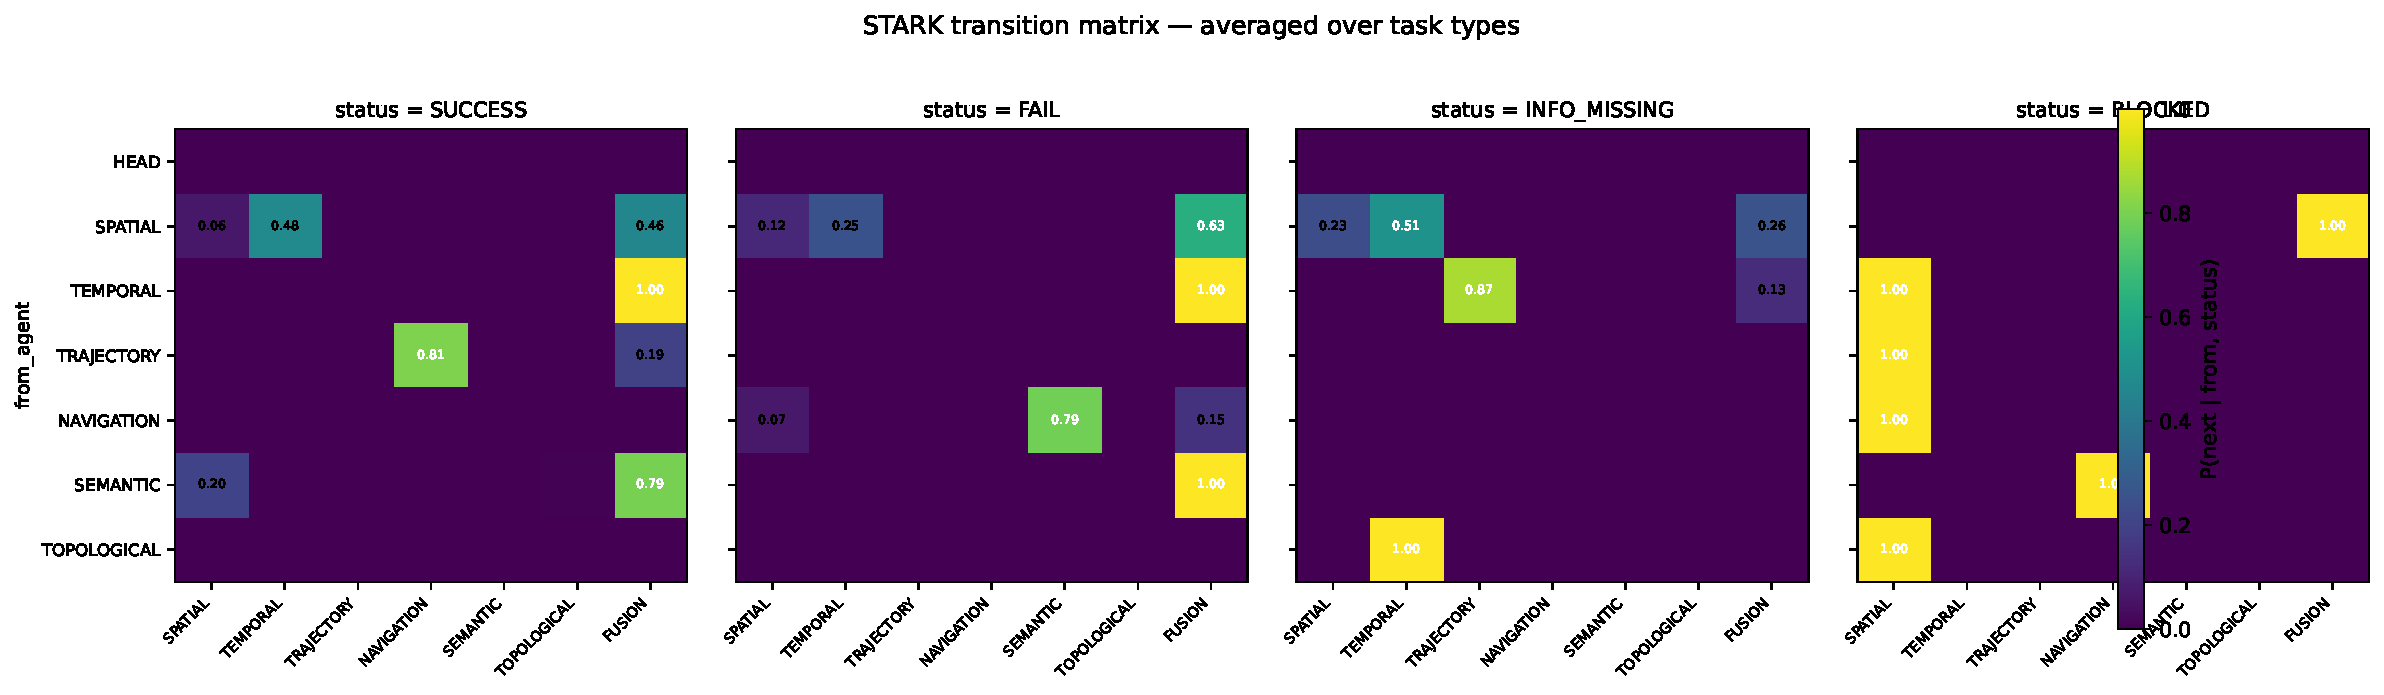
\includegraphics[width=\linewidth]{figures/matrix_heatmap_stark.pdf}
    \caption{STARK.}
    \label{fig:heatmap_stark}
\end{subfigure}

\vspace{0.35em}

\begin{subfigure}[b]{\textwidth}
    \centering
    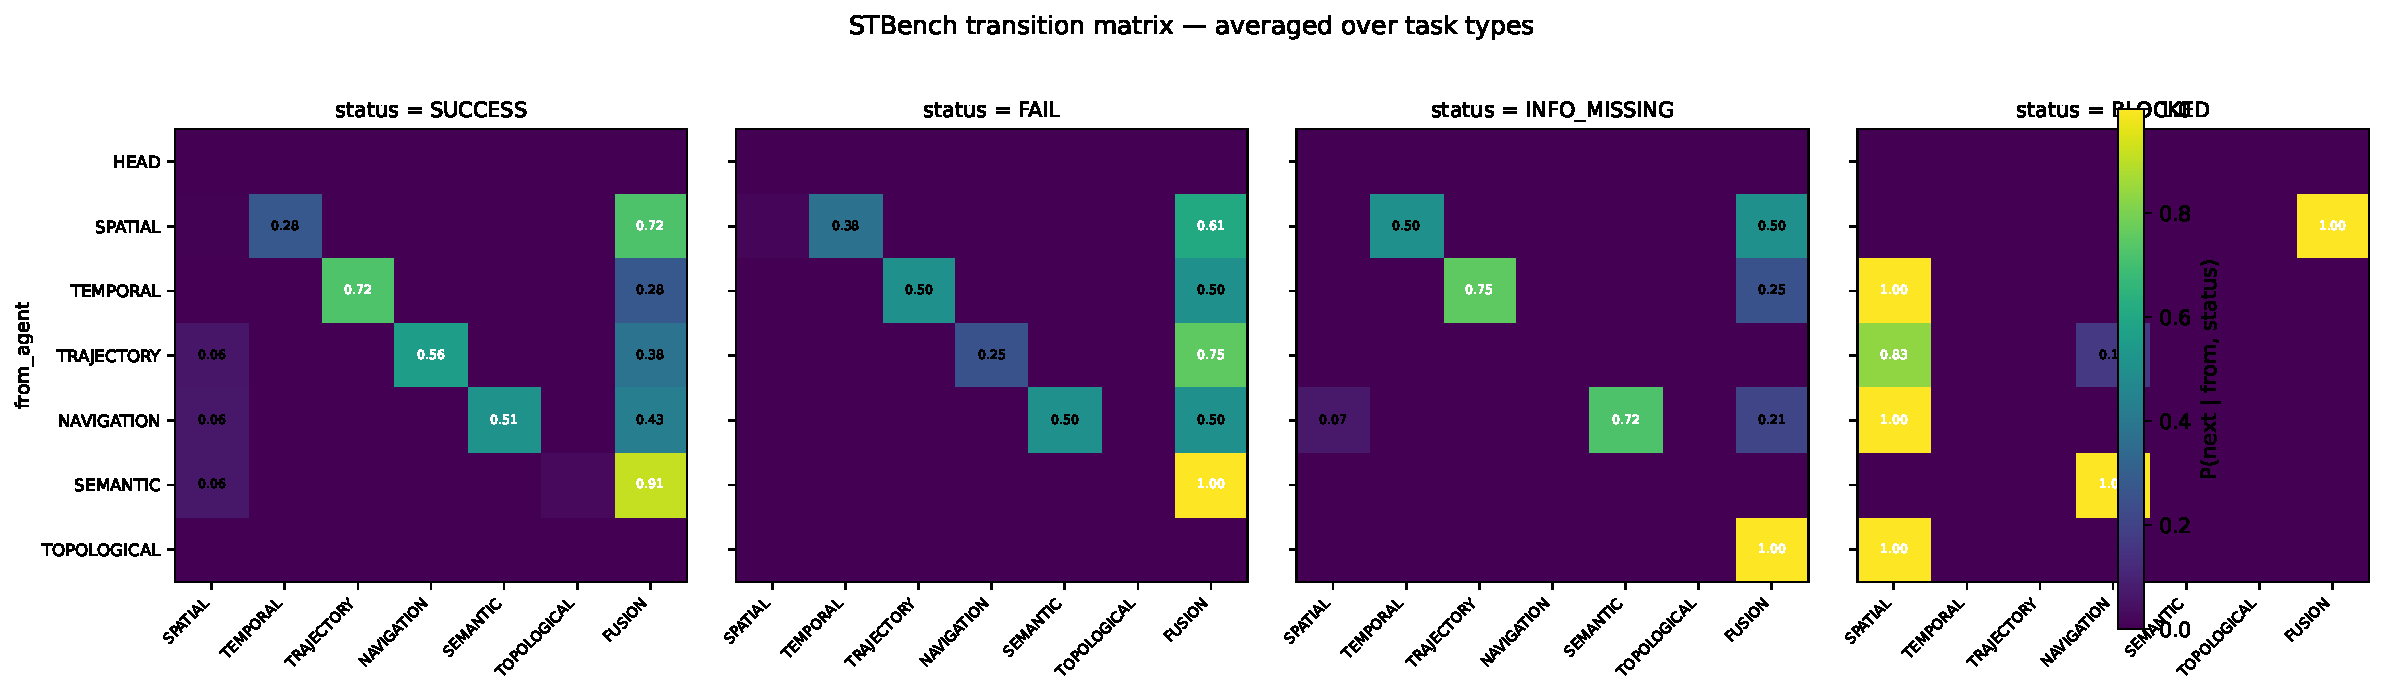
\includegraphics[width=\linewidth]{figures/matrix_heatmap_stbench.pdf}
    \caption{STB24.}
    \label{fig:heatmap_stbench}
\end{subfigure}

\vspace{0.35em}

\begin{subfigure}[b]{\textwidth}
    \centering
    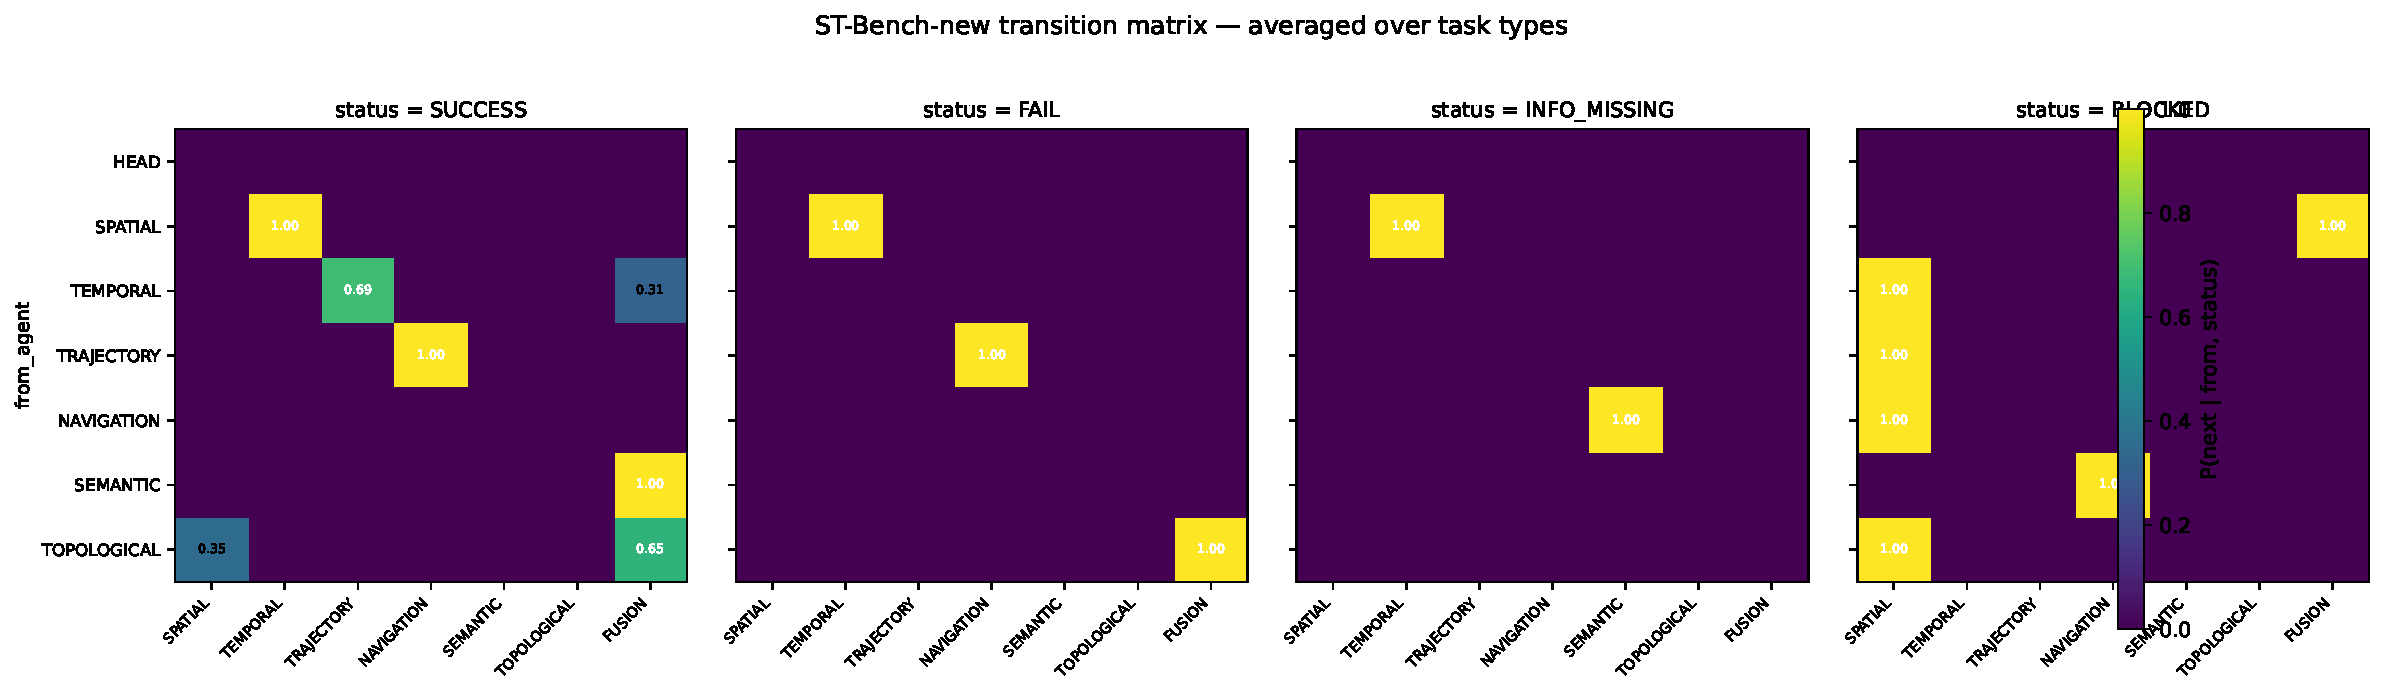
\includegraphics[width=\linewidth]{figures/matrix_heatmap_st_bench_new.pdf}
    \caption{STB26.}
    \label{fig:heatmap_stbenchnew}
\end{subfigure}
\caption{Learned transition matrix $\mathbf{M}$ averaged across task types, rendered as four status-conditional heatmaps (SUCCESS / FAIL / INFO\_MISSING / BLOCKED).  Rows index the \emph{from\_agent}, columns index the \emph{to\_agent}, and each cell is $P(\textit{next}\mid \textit{from}, \textit{status})$.  Each benchmark produces a qualitatively different SUCCESS map (because task taxonomies differ), but every benchmark exhibits the same structural property---error-state rows have non-zero support concentrated on different successors from the SUCCESS row, which is only possible because unsuccessful traces are retained during training (Theorem~\ref{thm:recovery}).  BLOCKED transitions are populated by the hand-curated safety-net table in System~1 plus any task-specific BLOCKED rules present in the matrix.}
\label{fig:matrix_heatmaps}
\end{figure}

\begin{figure}[p]
\centering
\begin{subfigure}[b]{\textwidth}
    \centering
    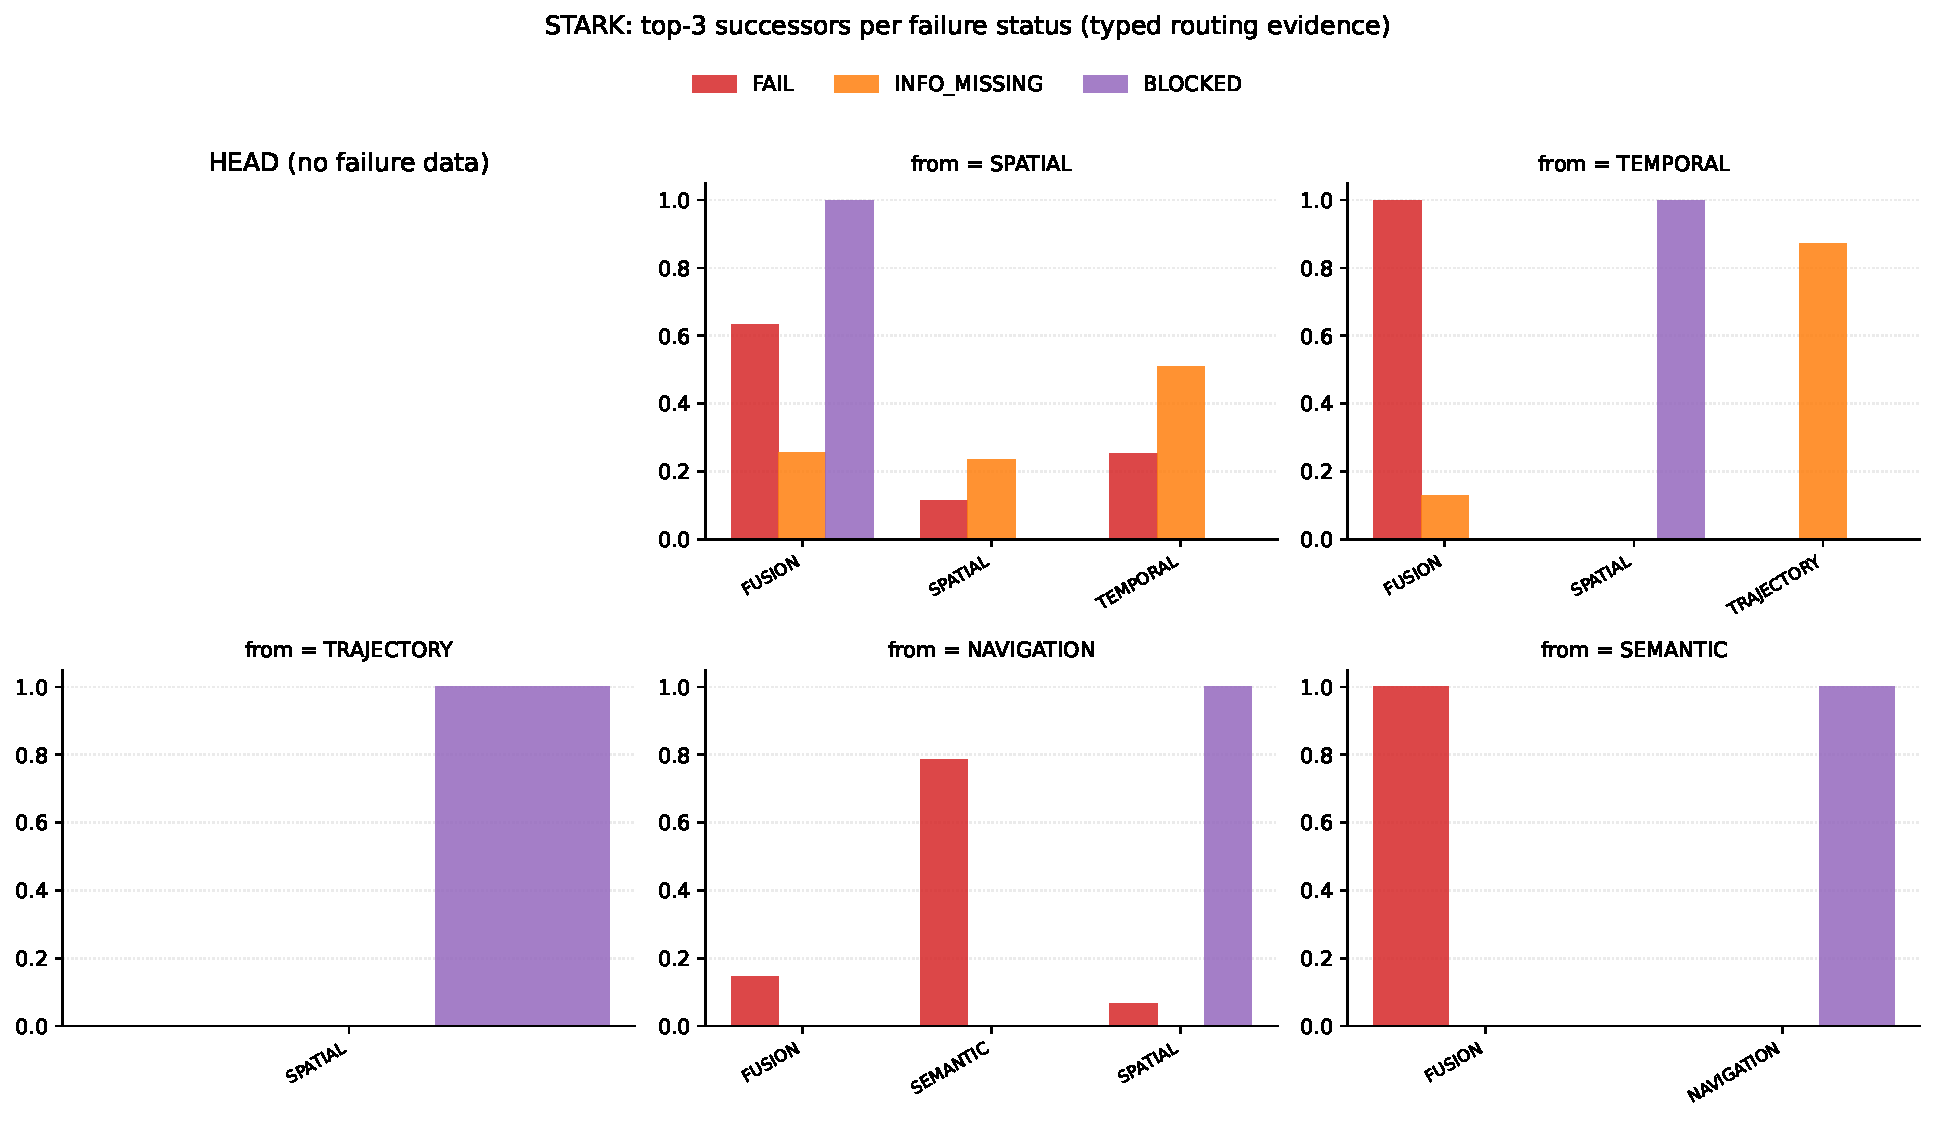
\includegraphics[width=0.72\linewidth]{figures/matrix_topk_stark.pdf}
    \caption{STARK.}
    \label{fig:topk_stark}
\end{subfigure}

\vspace{0.35em}

\begin{subfigure}[b]{\textwidth}
    \centering
    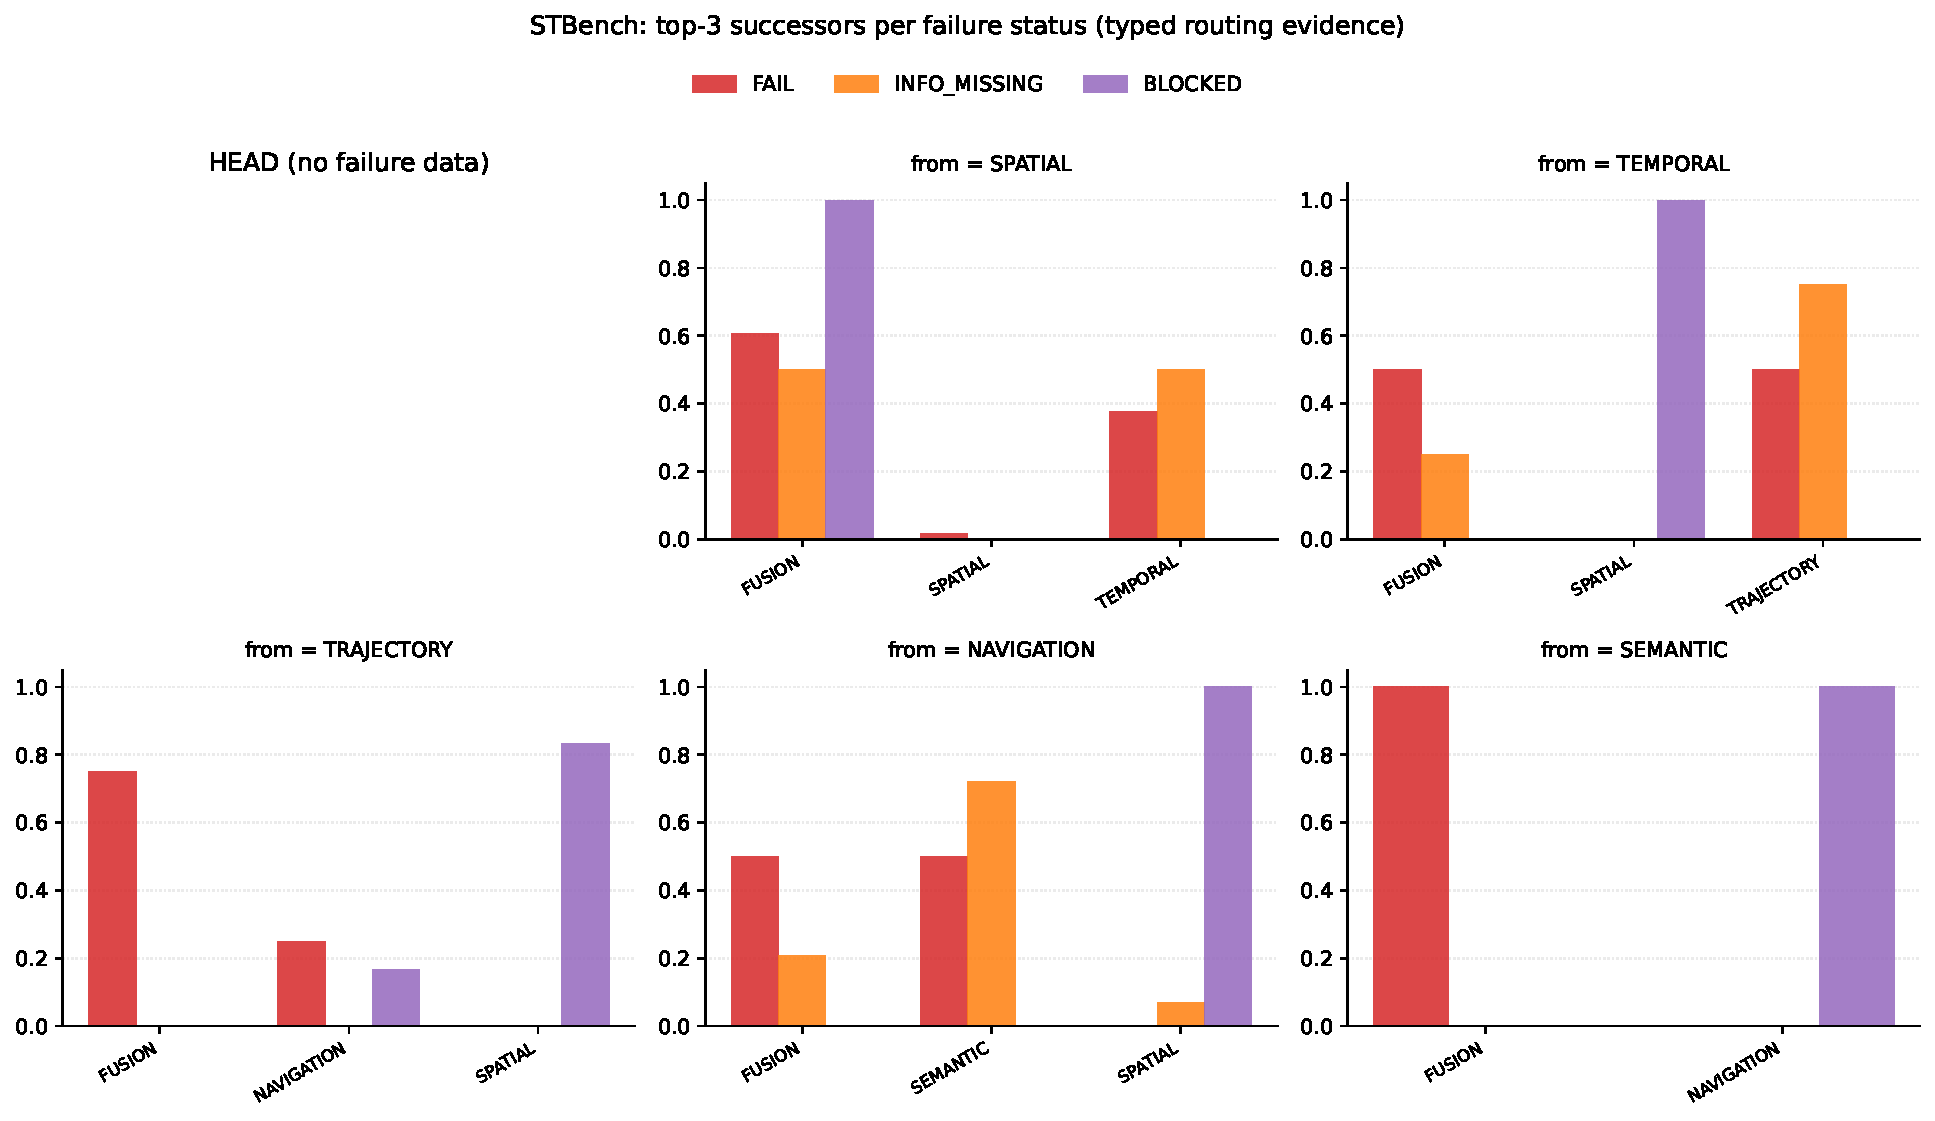
\includegraphics[width=0.72\linewidth]{figures/matrix_topk_stbench.pdf}
    \caption{STB24.}
    \label{fig:topk_stbench}
\end{subfigure}

\vspace{0.35em}

\begin{subfigure}[b]{\textwidth}
    \centering
    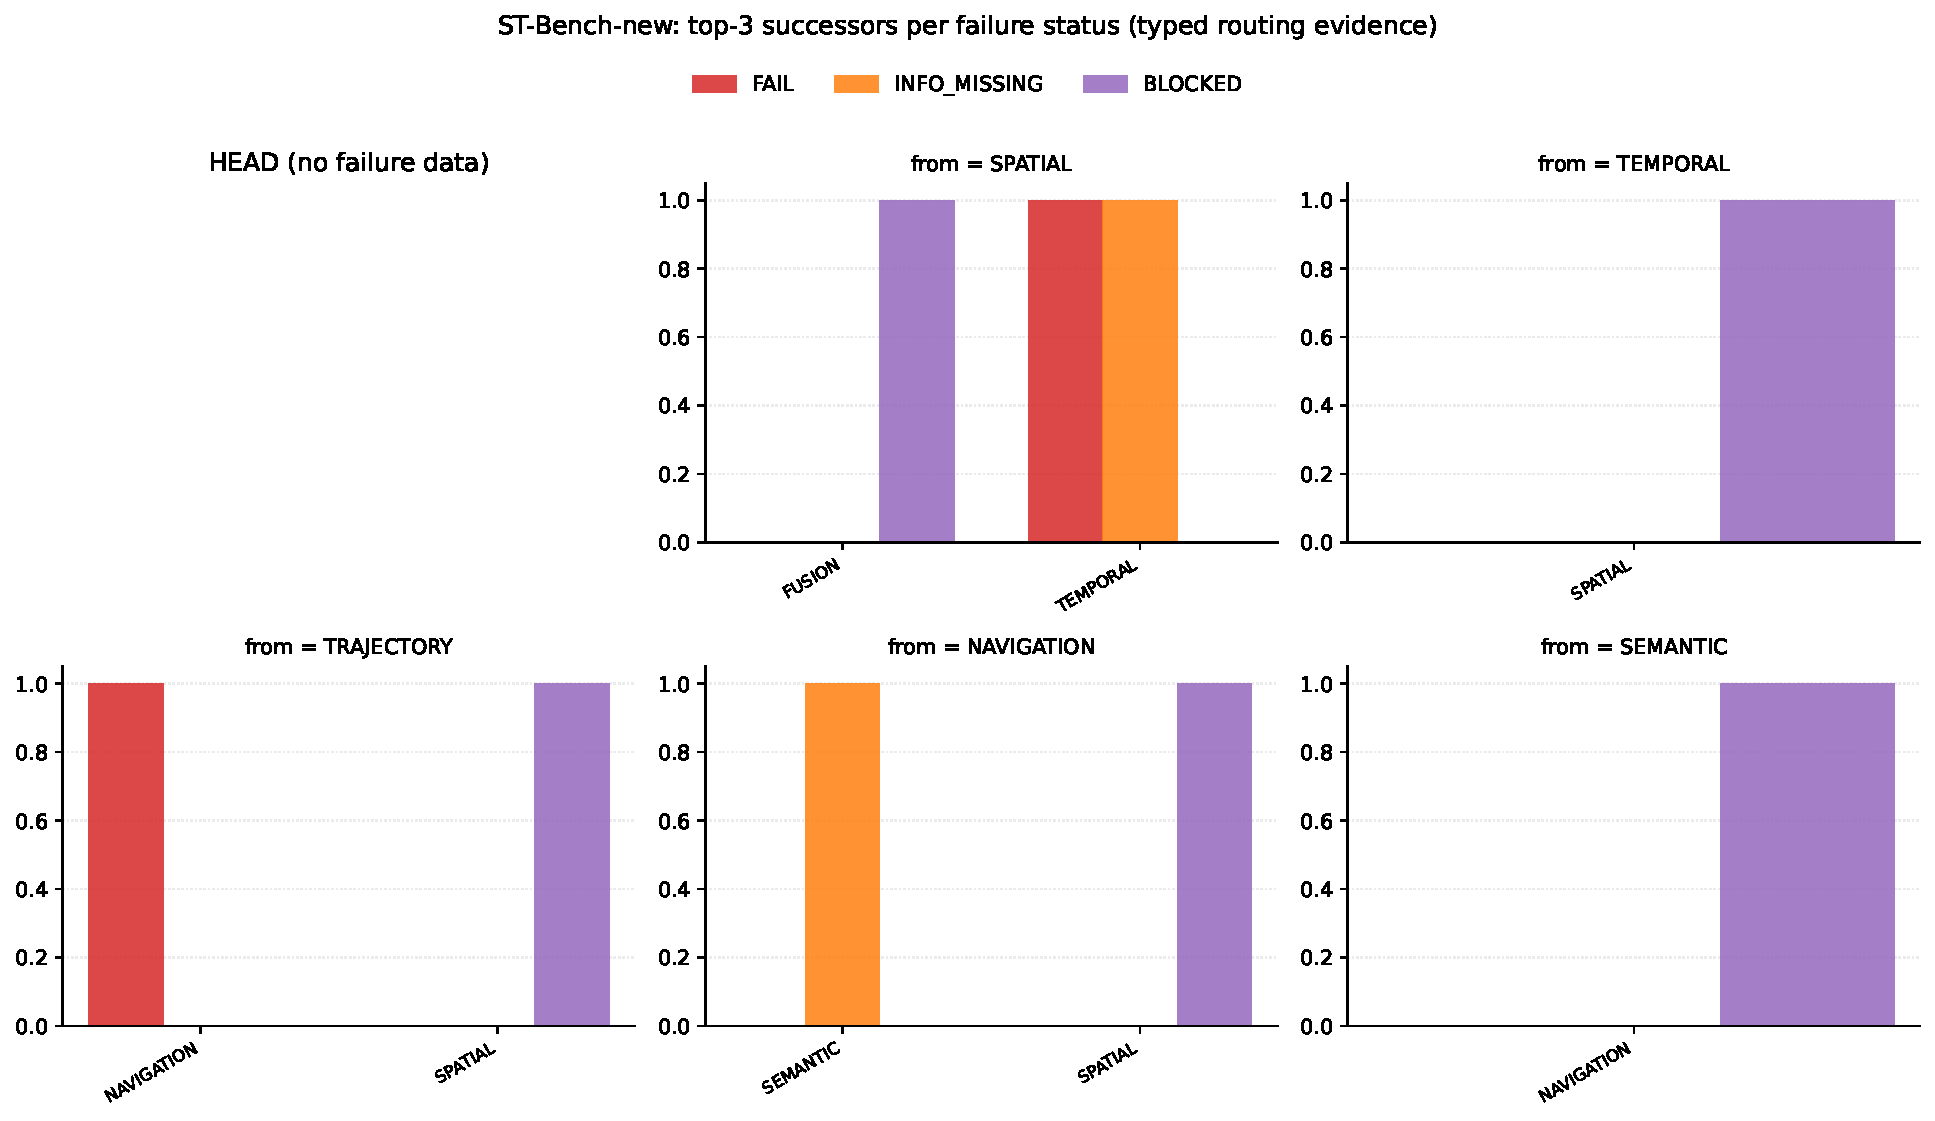
\includegraphics[width=0.72\linewidth]{figures/matrix_topk_st_bench_new.pdf}
    \caption{STB26.}
    \label{fig:topk_stbenchnew}
\end{subfigure}
\caption{Top-3 successors per failure status, grouped by originating agent.  For every \emph{from\_agent} in each benchmark, the three bars per successor show $P(\textit{next}\mid \textit{from}, \textit{status})$ for $\textit{status} \in \{\sfail, \smiss, \sblock\}$.  The claim visualized here is that the \emph{same} $(\textit{from\_agent}, \textit{task\_type})$ routes to \emph{different} recovery agents depending on the observed error type---the height pattern shifts across the three colored bars within each group.  This is the direct empirical counterpart of the status-conditioning ablation in Table~\ref{tab:router_ablation} (row ``No status conditioning''), which collapsed these three bars into one and paid up to 33pp on diverging STARK queries.}
\label{fig:matrix_topk}
\end{figure}


%% ============================================================
\FloatBarrier
\section{Composite Query Case Studies}
\label{app:composite}

Two composite query traces showing the full pipeline: HEAD decomposition $\to$ parallel agent execution $\to$ blackboard merge $\to$ multi-part FUSION.

\begin{table*}[!htbp]
\centering
\caption{\textbf{Composite Case 1}: Insurance claim verification (Event Analysis, SPATIAL+TEMPORAL).  Query: \textit{Is the vehicle trajectory within the parking zone? Does the claimed time window [1.5, 4.5] fall during the active window [0.0, 6.0]?}  GT: spatial=1, temporal=1.}
\label{tab:comp_case1}
\small
\begin{tabular}{c l p{9.5cm}}
\toprule
Step & Component & Trace \\
\midrule
1 & HEAD &
\texttt{LLM:} \texttt{\{"sub\_types": ["SPATIAL", "TEMPORAL"], "reasoning": "spatial analysis + temporal analysis"\}} \\
\midrule
2a & SPATIAL \newline (parallel) &
\texttt{LLM:} \texttt{<JSON>\{"operation": "within", "geom\_1": [[2.5,3.0],\ldots,[5.0,5.0]], "geom\_1\_type": "linestring", "geom\_2": [[2.0,2.0],\ldots,[2.0,2.0]], "geom\_2\_type": "polygon", "compute\_event\_interval": true\}</JSON>} \newline
\textbf{Tool}: \texttt{check\_within} $\to$ \texttt{True}. Event interval: [1.0, 5.0]. \\
\midrule
2b & TEMPORAL \newline (parallel) &
\texttt{LLM:} \texttt{<JSON>\{"relation": "overlaps", "interval\_1": [1.5, 4.5], "interval\_2": [0.0, 6.0]\}</JSON>} \newline
\textbf{Tool}: Allen's \texttt{during([1.5,4.5], [0.0,6.0])} $\to$ \texttt{True}. \\
\midrule
& $\Board$ &
\texttt{spatial\_data: \{within: True, event\_interval: [1.0, 5.0]\}} \newline
\texttt{temporal\_data: \{relation\_holds: True\}} \\
\midrule
3 & FUSION &
Reads both results $\to$ \texttt{\{"part1": 1, "part2": 1\}} \\
\midrule
& \textbf{Route} & HEAD $\to$ [SPATIAL $\|$ TEMPORAL] $\to$ FUSION \hfill \textbf{Both parts correct} $\checkmark$ \\
\bottomrule
\end{tabular}
\end{table*}

\begin{table*}[!htbp]
\centering
\caption{\textbf{Composite Case 2}: Weather monitoring (Event Analysis, SPATIAL+TEMPORAL).  Query: \textit{Does the storm trajectory intersect the sensor area? Does the storm's time [1.0, 3.0] overlap with maintenance [1.0, 2.5]?}  GT: spatial=1, temporal=1.}
\label{tab:comp_case2}
\small
\begin{tabular}{c l p{9.5cm}}
\toprule
Step & Component & Trace \\
\midrule
1 & HEAD &
\texttt{LLM:} \texttt{\{"sub\_types": ["SPATIAL", "TEMPORAL"], "reasoning": "spatial intersection + temporal overlap analysis"\}} \\
\midrule
2a & SPATIAL \newline (parallel) &
\texttt{LLM:} \texttt{<JSON>\{"operation": "intersects", "geom\_1": [[1.0,8.0],\ldots,[5.0,4.0]], "geom\_1\_type": "linestring", "geom\_2": [[2.5,4.5],\ldots,[2.5,4.5]], "geom\_2\_type": "polygon"\}</JSON>} \newline
\textbf{Tool}: \texttt{check\_intersects} $\to$ \texttt{True}. \\
\midrule
2b & TEMPORAL \newline (parallel) &
\texttt{LLM:} \texttt{<JSON>\{"relation": "overlaps", "interval\_1": [1.0, 3.0], "interval\_2": [1.0, 2.5]\}</JSON>} \newline
\textbf{Tool}: Allen's \texttt{overlaps([1.0,3.0], [1.0,2.5])} $\to$ \texttt{False} (starts equal, not strictly overlaps). \\
\midrule
& $\Board$ &
\texttt{spatial\_data: \{intersects: True\}}, \texttt{temporal\_data: \{overlaps: False\}} \\
\midrule
3 & FUSION &
Reads both $\to$ \texttt{\{"part1": 1, "part2": 0\}} \hfill (part2 incorrect: GT=1) \\
\midrule
& \textbf{Route} & HEAD $\to$ [SPATIAL $\|$ TEMPORAL] $\to$ FUSION \hfill \textbf{Partial: 1/2 correct} \\
\bottomrule
\end{tabular}
\end{table*}

\paragraph{Analysis.}
Case~1 demonstrates perfect multi-agent collaboration: HEAD decomposes into [SPATIAL, TEMPORAL], both agents execute in parallel, and FUSION synthesizes both parts correctly.
Case~2 shows an interesting error mode: the TEMPORAL agent selects Allen's \texttt{overlaps} but the intervals [1.0, 3.0] and [1.0, 2.5] share a start point, making the strict Allen relation \texttt{False}---the correct relation is \texttt{starts} (one interval starts at the same point and extends beyond).
This is a parameter extraction error (the LLM selected the wrong Allen relation), not a tool or routing error.

\paragraph{Agent activation patterns.}
Across all 14 composite queries, the HEAD agent correctly identifies the needed agent types in the majority of cases.
Trajectory monitoring queries (4/4) achieve correct decomposition into [TRAJECTORY, SPATIAL] with both agents returning $\ssucc$, yielding 75\% overall accuracy.
Event analysis achieves 70\% partial accuracy---spatial sub-parts are always correct, while temporal sub-parts occasionally fail due to Allen relation selection errors.
Logistics queries are limited by the navigation agent's ability to parse natural-text graph descriptions.

%% ============================================================
\FloatBarrier
\section{Case Studies with Full Traces}
\label{app:cases}

This section presents five worked examples drawn directly from benchmark test splits and the corresponding \starname{} execution traces recorded during the Qwen3-8B evaluation.  Each case reports:
(i) the raw query id and source file,
(ii) an excerpt of the query text as it enters the \shead{} agent (verbatim apart from whitespace cleanup),
(iii) the ground-truth answer,
(iv) the step-by-step trace including each agent's parameter-extraction JSON, the deterministic tool call, the blackboard update, and the final \sfuse{} synthesis.
Prompts are shortened with ``\texttt{[\ldots]}'' where truncated; JSON fields and numeric values are reproduced from the actual trace files.
The five cases are selected to cover (A)~a single-tool success, (B)~multi-agent blackboard composition, (C)~external-API tool use, (D)~\smiss-driven System~2 recovery, and (E)~graph-structured reasoning on the STB26 benchmark.

\subsection{Case A --- Single-tool success (STB24, Direction Determination)}
\label{app:case_a}

\textbf{Source.} \texttt{data/splits/stbench\_test.jsonl}, id \texttt{\seqsplit{stbench\_basic\_direction\_determination\_2261}}.
\textbf{Task type.} \texttt{STBENCH\_DIRECTION\_DETERMINATION}.
\textbf{Ground truth.} \texttt{1}.

\textbf{Raw query (verbatim).}
\begin{quote}\small\ttfamily
Question: A has a longitude of 120.1204 and a latitude of 30.8661, while B has a longitude of 128.3270 and a latitude of 45.458311. Therefore, B is in the () from A. Please choose the correct answer from the following options and fill it in parentheses. (1) North, (2) Northeast, (3) East, (4) Southeast, (5) South, (6) Southwest, (7) West, (8) Northwest. Please directly give me the number of your option with no other texts. Answer: Option (
\end{quote}

\begin{table}[H]
\centering
\caption{\textbf{Case~A}: execution trace.  Route: $\shead \xrightarrow{\ssucc} \ssp \xrightarrow{\ssucc} \sfuse$; predicted \texttt{1} $=$ GT.}
\label{tab:case_a}
\small
\begin{tabular}{c l p{10.5cm}}
\toprule
Step & Component & Trace \\
\midrule
1 & \shead{} &
\textit{System prompt.} Classify the query into exactly one \texttt{task\_type} from the 26-element catalog and emit \texttt{<JSON>\ldots</JSON>}. \newline
\textit{Model output.} \texttt{<JSON>\{"task\_type": "\seqsplit{STBENCH\_DIRECTION\_DETERMINATION}", "constraints": ["compass direction", "point coordinates"], "benchmark": "STBench"\}</JSON>} \newline
System~1 lookup for this \texttt{task\_type} $\Rightarrow$ primary agent $=$ \ssp{}. \\
\midrule
2 & \ssp{} &
\textit{Extraction prompt.} ``Pick one operation from: contains, crosses, intersects, within, touches, overlaps, equals, compass\_direction, haversine\_distance, landmark\_direction, admin\_region\_lookup, compute\_event\_interval, localization''. \newline
\textit{Model output.} \texttt{<JSON>\{"operation": "compass\_direction", "geom\_1": [120.1204, 30.8661], "geom\_2": [128.3270, 45.458311], "coordinates\_resolved": true\}</JSON>} \\
\midrule
  & Tool &
\texttt{tools.spatial\_ops.compute\_compass\_direction((120.1204, 30.8661), (128.3270, 45.458311))} returns bearing $\approx 27.3^{\circ}$ (clockwise from north) $\mapsto$ wedge (1)~North. \\
\midrule
  & $\Board$ update &
\texttt{spatial\_data = \{"direction\_result": 1, "bearing\_deg": 27.3\}} \\
\midrule
3 & \sfuse{} &
Reads \texttt{spatial\_data.direction\_result}, formats per task-type template $\Rightarrow$ \texttt{<answer>1</answer>}. \\
\bottomrule
\end{tabular}
\end{table}
\FloatBarrier
\subsection{Case B --- Multi-agent composition via blackboard (STARK, Spatiotemporal Relationship)}
\label{app:case_b}

\textbf{Source.} \texttt{data/splits/stark\_test.jsonl}, id \texttt{\seqsplit{stark\_Linestring\_Polygon\_within-during\_27}}.
\textbf{Task type.} \texttt{STARK\_SPATIOTEMPORAL\_RELATIONSHIP}.
\textbf{Ground truth.} \texttt{[0.0]} (relation does \emph{not} hold).

\textbf{Raw query (excerpt, non-boilerplate portion).}
\begin{quote}\small\ttfamily
Objective: Determine whether the time interval during which the EVENT holds has the temporal relationship \textbf{during} with the reference interval (6.5003, 11.8556)?

EVENT: the following object trajectory has the spatial relationship \textbf{within} with Polygon [(3.1253, 9.5958), (0.3137, 11.2892), (-2.1656, 9.1386), (-0.8864, 6.1160), (2.3836, 6.3986), (3.1253, 9.5958)]

Object trajectory: [(0.0000, 10.0000), (0.0826, 9.7639), (0.1701, 9.4990), (0.2650, 9.2067), (0.3698, 8.8887), (0.4865, 8.5477), (0.6172, 8.1864), (0.7636, 7.8081), (0.9269, 7.4164), (1.1082, 7.0153)]

Timestamp: [1.5770, 2.5974, 3.6178, 4.6382, 5.6586, 6.6790, 7.6994, 8.7198, 9.7402, 10.7606]

Answer 1 if Yes. Otherwise, answer 0.
[RESULTS\_START] [p] [RESULTS\_END]
\end{quote}

\begin{table}[H]
\centering
\caption{\textbf{Case~B}: multi-agent execution trace.  Route: $\shead \xrightarrow{\ssucc} \ssp \xrightarrow{\ssucc} \stp \xrightarrow{\ssucc} \sfuse$; predicted \texttt{[0.0]} $=$ GT.  The \ssp{} agent produces an intermediate \emph{event interval} that the \stp{} agent consumes from the blackboard --- without this composition the question is unanswerable by either agent alone.}
\label{tab:case_b}
\small
\begin{tabular}{c l p{10.5cm}}
\toprule
Step & Component & Trace \\
\midrule
1 & \shead{} &
\textit{Model output.} \texttt{<JSON>\{"task\_type": "\seqsplit{STARK\_SPATIOTEMPORAL\_RELATIONSHIP}", "constraints": ["spatial relation: within", "event interval", "temporal relation: during"], "benchmark": "STARK"\}</JSON>} \newline
System~1 $\Rightarrow$ primary $=$ \ssp{} (spatial predicate must be evaluated first so its event interval can feed \stp{}). \\
\midrule
2 & \ssp{} &
\textit{Extraction.} The agent must (i)~evaluate \texttt{within} pointwise, (ii)~project satisfying segments back to their timestamps, (iii)~emit the event interval. \newline
\textit{Model output.} \texttt{\seqsplit{<JSON>\{"operation": "within", "geom\_1": [[0.0,10.0],[0.083,9.76],[0.17,9.50],[0.27,9.21],[0.37,8.89],[0.49,8.55],[0.62,8.19],[0.76,7.81],[0.93,7.42],[1.11,7.02]], "geom\_1\_type": "linestring", "geom\_2": [[3.13,9.60],[0.31,11.29],[-2.17,9.14],[-0.89,6.12],[2.38,6.40],[3.13,9.60]], "geom\_2\_type": "polygon", "timestamps": [1.577, 2.597, 3.618, 4.638, 5.659, 6.679, 7.699, 8.720, 9.740, 10.761], "compute\_event\_interval": true\}</JSON>}} \\
\midrule
  & Tool &
\texttt{tools.spatial\_ops.within\_with\_event\_interval(traj, poly, timestamps)}.  Per-vertex Shapely within tests are all \texttt{True}; projecting first and last satisfying indices back yields event interval \texttt{[1.577, 10.761]}. \\
\midrule
  & $\Board$ update &
\texttt{spatial\_data = \{"spatial\_relation\_holds": True, "event\_interval": [1.577, 10.761]\}} \\
\midrule
3 & \stp{} &
\textit{Extraction.}  Reads \texttt{spatial\_data.event\_interval} from $\Board$; emits the Allen predicate. \newline
\textit{Model output.} \texttt{<JSON>\{"operation": "allen\_during", "interval\_a": [1.577, 10.761], "interval\_b": [6.5003, 11.8556]\}</JSON>} \\
\midrule
  & Tool &
\texttt{tools.temporal\_ops.allen\_during([1.577,10.761], [6.5003,11.8556])}: \emph{during}(A,B) requires $a_{\text{start}} > b_{\text{start}}$ and $a_{\text{end}} < b_{\text{end}}$. Here $1.577 < 6.5003$, so the relation is \texttt{False}. \\
\midrule
  & $\Board$ update &
\texttt{temporal\_data = \{"allen\_relation": "during", "holds": False\}} \\
\midrule
4 & \sfuse{} &
Reads both \texttt{spatial\_data.spatial\_relation\_holds}=True and \texttt{temporal\_data.holds}=False.  The task template requires both to hold for the combined relation $\Rightarrow$ answer $0$. Emits \texttt{[RESULTS\_START] [0.0] [RESULTS\_END]}. \\
\bottomrule
\end{tabular}
\end{table}
\FloatBarrier
\subsection{Case C --- External-API geocoding tool (STB24, Administrative Region)}
\label{app:case_c}

\textbf{Source.} \texttt{data/splits/stbench\_test.jsonl}, id \texttt{\seqsplit{stbench\_basic\_administrative\_region\_determination\_3977}}.
\textbf{Task type.} \texttt{STBENCH\_ADMIN\_REGION}.
\textbf{Ground truth.} \texttt{4}.

\textbf{Raw query (verbatim).}
\begin{quote}\small\ttfamily
Question: Below is the coordinate location information, and the options of the area where the coordinate may be located:
\{"latitude": 39.9407892, "longitude": -75.2596751,
 "options": "(0): Newport, PA (1): Presto, PA (2): Sturgeon, PA (3): Fogelsville, PA (4): Lansdowne, PA"\}
Please answer which area the coordinate is located in. Please just answer the number of your option with no other texts.
Answer: Option (
\end{quote}

\begin{table}[H]
\centering
\caption{\textbf{Case~C}: external-API tool trace.  Route: $\shead \xrightarrow{\ssucc} \ssp \xrightarrow{\ssucc} \sfuse$; predicted \texttt{4} $=$ GT.}
\label{tab:case_c}
\small
\begin{tabular}{c l p{10.5cm}}
\toprule
Step & Component & Trace \\
\midrule
1 & \shead{} &
\textit{Model output.} \texttt{<JSON>\{"task\_type": "STBENCH\_ADMIN\_REGION", "constraints": ["lat/lon coordinate", "5 candidate PA municipalities"], "benchmark": "STBench"\}</JSON>} \\
\midrule
2 & \ssp{} &
\textit{Extraction.}  \texttt{<JSON>\{"operation": "admin\_region\_lookup", "coordinates": [\{"latitude": 39.9407892, "longitude": -75.2596751\}], "options": ["Newport, PA", "Presto, PA", "Sturgeon, PA", "Fogelsville, PA", "Lansdowne, PA"], "coordinates\_resolved": true\}</JSON>} \\
\midrule
  & Tool &
\texttt{tools.spatial\_ops.admin\_region\_lookup(39.9408, -75.2597)}: reverse-geocodes via Nominatim, returns \texttt{"East Lansdowne, Delaware County, Pennsylvania, USA"}.  A rapidfuzz partial-ratio match against the five options scores ``Lansdowne, PA'' at 0.91, others $< 0.3$ $\Rightarrow$ option \texttt{4}. \\
\midrule
  & $\Board$ update &
\texttt{spatial\_data = \{"geocoded\_name": "East Lansdowne, Delaware County, Pennsylvania, USA", "matched\_option": 4, "match\_score": 0.91\}} \\
\midrule
3 & \sfuse{} &
Reads \texttt{matched\_option}, emits \texttt{<answer>4</answer>}. \\
\bottomrule
\end{tabular}
\end{table}
\FloatBarrier
\subsection{Case D --- \smiss{}-driven System~2 recovery (STARK, Landmark Direction)}
\label{app:case_d}

\textbf{Source.} \texttt{data/splits/stark\_test.jsonl}, id \texttt{stark\_direction\_questions\_37}.
\textbf{Task type.} \texttt{STARK\_LANDMARK\_DIRECTION}.
\textbf{Ground truth.} \texttt{[1.0]} (the proposed direction holds).

\textbf{Raw query (non-boilerplate portion).}
\begin{quote}\small\ttfamily
Objective: Determine the most accurate spatial relationship between Alcatraz Island, San Francisco, CA and Union Square, San Francisco, CA is south of, selecting from the options: ['north of', 'south of', 'east of', 'west of', 'north-east of', 'north-west of', 'south-east of', 'south-west of'].  The first location (A) is the reference location.  The direction tells you where B is with respect to that reference.  Answer 1 if answer is Yes. Otherwise, answer 0.
[RESULTS\_START] [p] [RESULTS\_END]
\end{quote}

\begin{table}[H]
\centering
\caption{\textbf{Case~D}: recovery via \smiss.  Route: $\shead \xrightarrow{\ssucc} \ssp \xrightarrow{\smiss} \sfuse_{\text{Sys.~2}}$; predicted \texttt{[1.0]} $=$ GT.  The primary \ssp{} call cannot resolve named landmarks without a gazetteer of SF points of interest, so it emits \smiss{} rather than fabricating coordinates.  The System~2 row of the transition matrix routes $(\ssp, \smiss, \texttt{STARK\_LANDMARK\_DIRECTION}) \mapsto \sfuse$ because the query text alone is sufficient for a world-knowledge answer.}
\label{tab:case_d}
\small
\begin{tabular}{c l p{10.5cm}}
\toprule
Step & Component & Trace \\
\midrule
1 & \shead{} &
\texttt{<JSON>\{"task\_type": "STARK\_LANDMARK\_DIRECTION", "constraints": ["named landmark pair", "compass wedge"], "benchmark": "STARK"\}</JSON>} \\
\midrule
2 & \ssp{} &
\textit{Extraction.}  \texttt{<JSON>\{"operation": "landmark\_direction", "geom\_1": "Alcatraz Island, San Francisco, CA", "geom\_2": "Union Square, San Francisco, CA", "proposed\_direction": "south of", "coordinates\_resolved": false\}</JSON>} \newline
Because \texttt{coordinates\_resolved=false} and no \texttt{navigation\_data.poi\_registry} entry is available on $\Board$ for either name, the agent returns \texttt{AgentResult(INFO\_MISSING, \{"missing": "landmark\_coordinates", "raw\_names": ["Alcatraz Island, San Francisco, CA", "Union Square, San Francisco, CA"]\})}. \\
\midrule
  & $\Board$ update &
\texttt{spatial\_data = \{"status": "INFO\_MISSING", "raw\_query\_echo": "Is Union Square south of Alcatraz Island?"\}} \\
\midrule
3 & Router &
System~1 exhausted for this \texttt{task\_type}; System~2 looks up $\mathbf{M}[\texttt{STARK\_LANDMARK\_DIRECTION}, \ssp, \smiss, \cdot]$.  The largest-mass successor is \sfuse{} (trained on traces where the LLM answered from background knowledge after tool failure).  The router dispatches \sfuse{} directly. \\
\midrule
4 & \sfuse{} &
Consumes the raw query plus the ``tool could not resolve landmarks'' flag.  Uses world knowledge that Union Square ($37.788^{\circ}$N) lies south of Alcatraz Island ($37.827^{\circ}$N), so ``south of'' is correct. \newline
\textit{Model output.} \texttt{[RESULTS\_START] [1.0] [RESULTS\_END]}. \\
\bottomrule
\end{tabular}
\end{table}
\FloatBarrier
\subsection{Case E --- Graph-structured etiological reasoning (STB26, Etiological MCQ)}
\label{app:case_e}

\textbf{Source.} \texttt{data/splits/st\_bench\_new\_test.jsonl}, id \texttt{st\_bench\_new\_5305}.
\textbf{Task type.} \texttt{ST\_BENCH\_NEW\_ETIOLOGICAL}.
\textbf{Ground truth.} \texttt{<answer>C</answer>}.

\textbf{Raw query (excerpt; all five 48-step time series are provided in full in the original prompt).}
\begin{quote}\small\ttfamily
You are a spatial temporal analysis expert.

Node 0 time series with length of 48: [300.7, 304.55, 290.54, 276.78, 272.19, 286.31, 291.35, 285.58, 302.58, 324.5, 321.06, \ldots, 271.54, 263.42];

Node 1 time series with length of 48: [348.36, 331.46, 327.99, 327.03, 315.48, 313.43, 307.54, 302.02, 307.6, 313.39, \ldots, 317.57, 305.87];

Node 2 \ldots{} [246.92, \ldots, 277.26];

Node 3 \ldots{} [275.33, \ldots, 287.06];

Node 4 \ldots{} [222.21, \ldots, 262.21];

Graph Structure: Node 0 $\to$ Node 1; Node 1 $\to$ Node 3; Node 2 $\to$ Node 1; Node 3 $\to$ Node 4; Node 4 $\to$ Node 2.

Question: Which etiological scenario can be inferred from the spatio-temporal data?

Options:
A.~Six-node logistics network measuring freight movement between industrial parks and distribution centers via expressways.
B.~Three-node public transit system monitoring passenger counts between airport terminals and suburban rail stations.
C.~Five-node urban transport network tracking traffic flow between CBD and residential areas through highway and arterial connections.
D.~Four-node metro system tracking passenger volume between university campuses and entertainment districts through underground lines.
\end{quote}

\begin{table}[H]
\centering
\caption{\textbf{Case~E}: graph-topology reasoning with deterministic structural filters.  Route: $\shead \xrightarrow{\ssucc} \stopo \xrightarrow{\ssucc} \sfuse$; predicted \texttt{<answer>C</answer>} $=$ GT.  Topology enumeration (node count, edge count, cycle presence) narrows the four options to a single survivor before the LLM is consulted.}
\label{tab:case_e}
\small
\begin{tabular}{c l p{10.5cm}}
\toprule
Step & Component & Trace \\
\midrule
1 & \shead{} &
\texttt{<JSON>\{"task\_type": "ST\_BENCH\_NEW\_ETIOLOGICAL", "constraints": ["5 nodes", "5 directed edges", "multivariate time series length 48", "4 MCQ options"], "benchmark": "ST-Bench-new"\}</JSON>} \\
\midrule
2 & \stopo{} &
\textit{Extraction.}  \texttt{<JSON>\{"operation": "analyze\_topology", "nodes": [0,1,2,3,4], "edges": [[0,1],[1,3],[2,1],[3,4],[4,2]], "series\_length": 48, "n\_series": 5, "mcq\_options": ["A: 6-node logistics", "B: 3-node transit", "C: 5-node urban transport", "D: 4-node metro"]\}</JSON>} \\
\midrule
  & Tool &
\texttt{tools.graph\_ops.analyze\_topology(nodes, edges)} returns \texttt{\{"n\_nodes":5, "n\_edges":5, "cyclic":true, "source":0, "longest\_path":[0,1,3,4,2], "centrality\_node":1\}}. \newline
\texttt{tools.graph\_ops.detect\_cascade(series, edges)} returns onset times \texttt{\{0:33, 1:14, 3:16, 4:38, 2:38\}} with propagation lag matching the edge directions. \newline
\textbf{MCQ structural filter.}  Option node-count $\{A:6, B:3, C:5, D:4\}$ vs.\ observed $n_{\text{nodes}}=5$ $\Rightarrow$ only option C matches.  Tool-side MCQ score vector becomes $\{A:0, B:0, C:1, D:0\}$ with confidence $1.0$. \\
\midrule
  & $\Board$ update &
\texttt{topological\_data = \{"n\_nodes":5, "cyclic":true, "matching\_options":["C"], "tool\_confidence":1.0, "cascade\_onsets": \{0:33, 1:14, 3:16, 4:38, 2:38\}\}} \\
\midrule
3 & \sfuse{} &
\textit{System prompt.}  ``You will be given topology summaries plus cascade evidence.  Select the single best option.'' \newline
Reads \texttt{matching\_options}$=$\texttt{[C]} with \texttt{tool\_confidence} $\geq 0.5$ $\Rightarrow$ emits \texttt{<answer>C</answer>} without invoking the LLM scoring fallback (which would only trigger if \texttt{tool\_confidence $< 0.5$}). \\
\bottomrule
\end{tabular}
\end{table}
\FloatBarrier

%% Force all remaining floats out before checklist
\clearpage
